%%%%%%%%%%%%%%%%%%%%%%%%%%%%%%%%%%%%%%%%%%%%%%%%%%%%%%%%%%%%%%%%%%%%%%%%%
%%   CHAPTER: PERIODIC CIRCUITRY
%%%%%%%%%%%%%%%%%%%%%%%%%%%%%%%%%%%%%%%%%%%%%%%%%%%%%%%%%%%%%%%%%%%%%%%%%

\renewcommand{\chapterfolder}{periodic_circuitry/}
\chapterimage{cover/periodic_circuitry}
\chapter{Periodic Circuitry}\label{chp:periodic_circuitry}


\vspace*{-0.4in}
\epigraph{Sometimes you're a glider, sometimes a spaceship, and sometimes just a hole.}{David Goodenough}
\vspace*{0.4in}


\noindent The breeder that we constructed in Section~\ref{sec:gosper_breeder} demonstrated a very important fact about how we will proceed with Life from this point on---we typically construct large patterns that do unusual things via a two-step process:\smallskip

\begin{enumerate}
	\item[1)] First, we design a ``schematic'' that illustrates the rough shape of the object and where the gliders (our standard building blocks) will travel. For example, for the breeder we wanted to construct a pattern that synthesizes an endless row of Gosper glider guns. We thus need the source of gliders that create those guns to move (i.e., we need them to come from rakes), so we reasonably quickly arrive at the schematic shown in Figure~\ref{fig:ggg_breeder_schematic}.\bigskip
	
	\noindent\begin{minipage}{\linewidth}
		\centering
		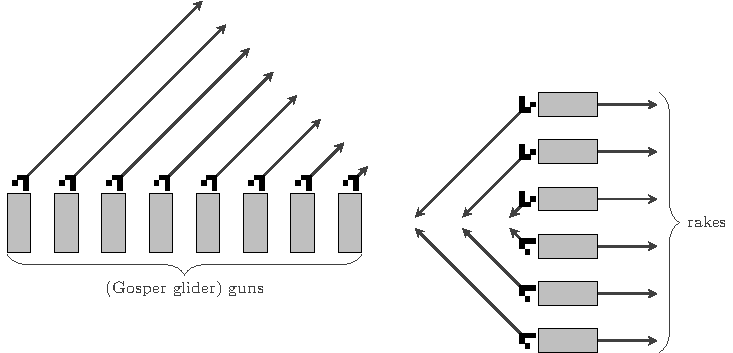
\includegraphics[width=0.9\textwidth]{periodic_circuitry/breeder_schematic.pdf}
		\captionof{figure}{A schematic that gives a rough picture of how the breeder that we constructed in Section~\ref{sec:gosper_breeder} works.}\label{fig:ggg_breeder_schematic}\bigskip
	\end{minipage}
	
	\item[2)] Next, we fill in the details---we place guns, rakes, reflectors, and other components that actually make the gliders (and potentially other spaceships) follow the tracks indicated and perform the required syntheses. For example, when constructing the breeder in Section~\ref{sec:gosper_breeder}, we arranged a total of $12$ period~$60$ space rakes at the right-hand-side of the pattern to carry out the indicated Gosper glider gun synthesis.\smallskip
\end{enumerate}

Depending on the complexity of the schematic, implementing the second step above might be rather tricky, as manipulating glider paths and timing can be a somewhat fiddly and time-consuming affair. In this chapter, our goal is to develop circuitry that can help us do exactly this. That is, we start introducing circuitry that makes it easier to move gliders (and other spaceships) around tracks in such a way that we can make them appear wherever we want, whenever we want.

For now, we focus on periodic circuitry based on oscillators. The advantage of this type of circuitry is that it is typically smaller and simpler than stationary circuitry (which we explore in the next chapter, and is instead based on still lifes). However, it has the disadvantage that it can be difficult or impossible to make circuitry based on different periods work together. For example, if a period-$5$ oscillator is used to reflect a glider in some part of a mechanism, then the glider stream we are working with must have a period that is a multiple of $5$, and all other connected circuitry must also work at the same period.


%%%%%%%%%%%%%%%%%%%%%%%%%%%%%%%%%%%%%%%%%%%%%%%%%%%%%%%%%%%%%%%%%%%%%%%%%
%%   SUBSECTION: P30 CIRCUITRY
%%%%%%%%%%%%%%%%%%%%%%%%%%%%%%%%%%%%%%%%%%%%%%%%%%%%%%%%%%%%%%%%%%%%%%%%%
\section{Period~30 Circuitry}\label{sec:p30}

The simplest set of circuitry that exists is based off of the queen bee shuttle and thus has period~$30$. For example, we already saw that we can use the queen bee shuttle to construct the Gosper glider gun (Figure~\ref{fig:ch6_ggg}) and buckaroo\index{buckaroo} (Figure~\ref{fig:buckaroo_reflect}), which create and reflect gliders, respectively. We now present some other oscillators and circuits with compatible periods that can be used in conjunction with period~$30$ glider streams, and we also investigate how we can use these objects to manipulate glider streams in even more exotic ways.


\begin{figure}[!htb]
	\centering
	\begin{minipage}[b]{0.48\textwidth}
		\centering
		\patternimg{0.125}{gosper_glider_gun}
		\caption{A Gosper glider gun producing gliders at a spacing of $30$~generations.}\label{fig:ch6_ggg}
	\end{minipage}\hfill
	\begin{minipage}[b]{0.48\textwidth}
		\centering
		\patternimg{0.125}{buckaroo_reflect}
		\caption{A buckaroo can reflect a glider by $90$~degrees, from the position marked in \bgbox{greenback}{green} to the one in \bgbox{orangeback}{orange} $30$ generations later.}\label{fig:buckaroo_reflect}
	\end{minipage}
\end{figure}


%%%%%%%%%%%%%%%%%%%%%%%%%%%%%%%%%%%%%%%%%%%%%%%%%%%%%%%%%%%%%%%%%%%%%%%%%
%%   SUBSECTION: P30 REFLECTION
%%%%%%%%%%%%%%%%%%%%%%%%%%%%%%%%%%%%%%%%%%%%%%%%%%%%%%%%%%%%%%%%%%%%%%%%%
\subsection{Reflectors}\label{sec:p30_reflectors}

Because the pentadecathlon\index{pentadecathlon} has period $15$, which is a divisor of $30$, it works very well with other period~$30$ circuitry. In particular, it can be used to reflect gliders in numerous different ways that are shown in Figure~\ref{fig:p30_reflectors}. The reflection shown in Figure~\ref{fig:p30_relay} is the same one that we saw back in the period~$60$ oscillator of Figure~\ref{fig:relay}, but the other two are new.

\begin{figure}[!htb]
	\centering
	\begin{tabular}{@{}ccc@{}}
		\begin{subfigure}{.31\textwidth}
			\centering\vspace*{1.91cm}
			\patternimg{0.14}{p30_relay}
			\caption{A pentadecathlon reflecting a glider by $180$~degrees.}
			\label{fig:p30_relay}
		\end{subfigure} &
		\begin{subfigure}{.31\textwidth}
			\centering
			\patternimglink{0.135}{p30_180_reflect}
			\caption{Two pentadecathlons reflecting a glider by $180$~degrees.}
			\label{fig:p30_180_reflect}
		\end{subfigure} &
		\begin{subfigure}{.31\textwidth}
			\centering
			\patternimglink{0.135}{p30_90_reflect_penta}
			\caption{Two pentadecathlons reflecting a glider by $90$~degrees.}
			\label{fig:p30_90_reflect_penta}
		\end{subfigure}
	\end{tabular}
	\caption{Some period~$15$ pentadecathlon-based reflectors that work well with glider streams whose period is a multiple of~$15$ (the reflector (c) requires period at least~$45$). Input gliders are \bgbox{greenback}{green}, while the location where they will be $30$ generations later is displayed in \bgbox{orangeback}{orange}.}
	\label{fig:p30_reflectors}
\end{figure}

In particular, Figure~\ref{fig:p30_180_reflect} shows how two pentadecathlons can be used as a $180$-degree reflector with slightly different timing and positioning than the one that we already knew about (i.e., the one in Figure~\ref{fig:p30_relay}), and Figure~\ref{fig:p30_90_reflect_penta} shows that two pentadecathlons can be used to create a $90$-degree color-preserving reflector. There are also a few other period~$30$-friendly ways to reflect gliders aside from using pentadecathlons and buckaroos. We will see some color-changing $90$-degree methods in Figures~\ref{fig:p15_bouncer} and~\ref{fig:p5_bouncer}, and two more color-preserving $90$-degree options in Exercises~\ref{exer:bumper_high_period}(c) and~\ref{exer:bumper_high_period}(d).\footnote{It is also trivially the case that stable reflectors work with glider streams whose period is a large enough multiple of~$30$ (at least~$60$ in the case of the Snark).} 


%%%%%%%%%%%%%%%%%%%%%%%%%%%%%%%%%%%%%%%%%%%%%%%%%%%%%%%%%%%%%%%%%%%%%%%%%
%%   SUBSECTION: P30 INVERSION
%%%%%%%%%%%%%%%%%%%%%%%%%%%%%%%%%%%%%%%%%%%%%%%%%%%%%%%%%%%%%%%%%%%%%%%%%
\subsection{Inverters}\label{sec:p30_inline_inverter}

If we have an \emph{irregular} glider stream---one in which gliders are separated by a fixed period, except some gliders are missing---it is often useful to invert the stream. That is, we would like to have a mechanism for replacing the gliders in the stream by empty gaps, and replacing the empty gaps by gliders.

One simple method of implementing this inversion (which works at any period) is to use a glider gun to fire a regular stream at the irregular stream so that gliders collide so as to annihilate each other. Then any gliders that are present in the irregular stream will be destroyed by the gun, while any gliders that are missing in the irregular stream will be generated by the gun, as illustrated in Figure~\ref{fig:inverter_non_inline}.

\begin{figure}[!htb]
	\centering
	\patternimglink{0.12}{inverter_non_inline}
	\caption{A glider stream (highlighted in \bgbox{greenpastel}{green}) can be inverted by a glider gun (highlighted in \bgbox{yellowback2}{yellow}). In this case, a p120 input stream is converted into a p30 output stream (highlighted in \bgbox{orangeback2}{orange}) that is missing one out of every four gliders.}
	\label{fig:inverter_non_inline}
\end{figure}

At period~30, there is a modification of this reaction that has the advantage that the irregular input stream and its inversion travel in the same direction. Recall that the Gosper glider gun works by colliding two queen bees with each other so that they create a small explosion that then generates a glider. If we carefully fire a glider at that small explosion, we can suppress its creation of a glider, resulting in a reaction called an \emph{inline inverter}\index{inline inverter}.\footnote{Discovered by David Bell. There are also inline inverters based on some other glider guns---see the upcoming Figure~\ref{fig:tanners_p46_inline_inverter}.} The output stream travels in the same direction as the input stream, but is slightly offset (see Figure~\ref{fig:inline_inverter_both}).

\begin{figure}[!htb]
	\centering
	\begin{tabular}{@{}ccc@{}}
		\begin{subfigure}{.46\textwidth}
			\centering
			\patternimglink{0.11}{inline_inverter}
			\caption{If an input glider is \emph{not} present then an output glider will appear at the location marked in \bgbox{orangeback}{orange} $30$ generations after the phase shown here (i.e., the output stream is $5$ cell further south than the input stream).}
			\label{fig:inline_inverter}
		\end{subfigure} &
		\begin{subfigure}{.51\textwidth}
			\centering
			\patternimglink{0.105}{inline_inverter_p120}
			\caption{An inline inverter converting a thin glider stream into a thick one. A period~$120$ glider stream is converted into a period~$30$ stream that is missing one out of every four gliders, just like in Figure~\ref{fig:inverter_non_inline}.}
			\label{fig:inline_inverter_p120}
		\end{subfigure}	
	\end{tabular}
	\caption{An \emph{inline inverter} is a reaction involving the Gosper glider gun in which the gun fails to produce a glider if it receives a glider as input at the same time.}
	\label{fig:inline_inverter_both}
\end{figure}

These inverters can be used to create many new types of patterns that we have not yet seen, such as glider guns with extremely large period. For example, we can use one Gosper glider gun to feed gliders into an inline inverter, creating a period~$30$ oscillator made up of a glider stream of any finite length of our choosing. We can then trigger this oscillator to release a glider by destroying one of the gliders in the central stream. For example, we can use one of the two-glider collisions from Table~\ref{tab:2_glider_synth} to have a glider bounce off of the glider stream, resulting in a single other glider escaping from the stream, as in Figure~\ref{fig:inline_inverter_bounce}.

\begin{figure}[!htb]
	\centering
	\embedlink{inline_inverter_bounce}{\vcenteredhbox{\patternimg{0.12}{inline_inverter_bounce}} \vcenteredhbox{\genarrow{15}} \vcenteredhbox{\patternimg{0.12}{inline_inverter_bounce_15}} \vcenteredhbox{\genarrow{15}} \vcenteredhbox{\patternimg{0.12}{inline_inverter_bounce_30}}}
	\caption{Two Gosper glider guns can be placed near each other so as to create a finite stream of gliders (highlighted here in \bgbox{aquaback}{aqua}) between them. Here, we bounce a single glider (in \bgbox{greenback}{green}) off of one of those gliders (in \bgbox{orangeback}{orange}) so that it is destroyed and thus released by the inline inverter to the southeast.}
	\label{fig:inline_inverter_bounce}
\end{figure}

By bouncing a glider back and forth between two of these finite-length glider streams, we can create glider guns with arbitrarily large periods. In particular, by shifting these two mechanisms away from each other by multiples of $15$ cells, we can create glider guns with period equal to $120n$ for any integer $n \geq 1$. Figure~\ref{fig:inverter_p120_gun_inline_and_not} illustrates some guns of this type with period~$120$.

% NJ: Removing this paragraph as it is now taken care of by the introduction of non-inline inverters at the start
%We should clarify at this point that there are actually many other methods of stream inversion possible as well, but these other methods typically result in the inverted stream being reflected by $90$~degrees from the input stream, rather than going in the same direction as it (i.e., the inversion is not ``inline''). For example, simply firing an irregular stream at a regular stream so that they collide as in one of the two-glider annihilations from Table~\ref{tab:2_glider_synth} results in an inverter. This inverter can do many of the same things as the inline inverter, such as creating high-period guns, as in Figure~\ref{fig:inverter_p120_gun}. If desired, we can turn this inversion into one that is inline simply by pairing it with any compatible 90-degree periodic reflector, or with a Snark as long as the period is $43$ or greater.

\begin{figure}[!htb]
	\centering
	\begin{subfigure}{.48\textwidth}
		\centering
		\patternimglink{0.084}{inline_inverter_p120_gun}
		\caption{p$120$ gun from inline inverter}
		\label{fig:inline_inverter_p120_gun}
	\end{subfigure} \ \ \ % 
	\begin{subfigure}{.49\textwidth}
		\centering
		\patternimglink{0.084}{inverter_p120_gun}
		\caption{p$120$ gun from collision-based non-inline inverter}
		\label{fig:inverter_p120_gun}
	\end{subfigure}
	\caption{Three Gosper glider guns (highlighted in \bgbox{yellowback2}{yellow}, the bottom of which acts as an inverter) can be used to create a period~$120$ glider gun. The glider displayed in \bgbox{greenback}{green} bounces back and forth between the two \bgbox{aquaback}{aqua} glider streams, destroying one glider in each stream every time it is reflected. The glider that is destroyed in the left stream is then created (in \bgbox{orangeback}{orange}) by the inverter. In (a) the bottom glider gun is an inline inverter, whereas in (b) it is a non-inline inverter.}\label{fig:inverter_p120_gun_inline_and_not}
\end{figure}

Another particularly useful inversion reaction is provided in Figure~\ref{fig:stream_inverter}, in which a glider stream of any period $20$ or larger collides with an \emph{irregular}\index{irregular stream} stream of the same period (i.e., a stream with some gliders potentially missing). If a glider is missing in the irregular glider stream, then the corresponding glider in the regular stream passes by unharmed. On the other hand, if a glider is present in the irregular glider stream, then a collision occurs that generates a glider in a different direction. There are thus two output glider streams: one that contains exactly the same gliders as the irregular input stream, and one that is the inverse of that stream (i.e., it contains a glider if and only if the irregular input stream did not).

\begin{figure}[!htb]
	\centering
	\begin{subfigure}{.48\textwidth}
		\centering
		\embedlink{stream_inverter}{\vcenteredhbox{\patternimg{0.12}{inverter0_0}} \vcenteredhbox{\genarrow{12}} \vcenteredhbox{\patternimg{0.12}{inverter0_12}}}
		\caption{This collision causes the top-right glider to be erased and the top-left glider to be slightly offset.}
		\label{fig:stream_inverter_yes}
	\end{subfigure} \ \ \ \ % 
	\begin{subfigure}{.48\textwidth}
		\centering
		\embedlink{stream_inverter}{\vcenteredhbox{\patternimg{0.12}{inverter1_0}} \vcenteredhbox{\genarrow{12}} \vcenteredhbox{\patternimg{0.12}{inverter1_12}}}
		\caption{If the top-left glider is omitted, the top-right glider passes by unharmed.}
		\label{fig:stream_inverter_no}
	\end{subfigure}
	\caption{A stream inverter that splits the glider stream coming in from the northeast based on which gliders are present in the stream coming in from the northwest. This reaction can be used with any glider stream of period~$20$ or higher. The output stream going to the southeast is a duplicate of the input stream coming from the northwest, whereas the output stream going to the southwest is its inverse.}\label{fig:stream_inverter}
\end{figure}

This reaction can thus be used as a \emph{non-destructive} inverter: it produces an inverted glider stream, but does not use up the original irregular stream in the process. By applying another inverter to the inverted stream that this reaction produces, we can now duplicate arbitrary glider streams (even irregular ones), as in Figure~\ref{fig:periodic_glider_duplicator}. Patterns like this one are called \emph{glider duplicators}\index{glider!duplicator}, and they are extremely important because they let us use a single input signal (i.e., a glider) to trigger multiple different reactions.

\begin{figure}[!htb]
	\centering
	\embedlink{glider_duplicator}{\vcenteredhbox{\patternimg{0.128}{glider_duplicator_0}} \vcenteredhbox{\genarrow{30}} \vcenteredhbox{\patternimg{0.128}{glider_duplicator_30}} \vcenteredhbox{\genarrow{60}} \vcenteredhbox{\patternimg{0.128}{glider_duplicator_90}}}
	\caption{A glider duplicator that makes use of the inline inverter and the reaction from Figure~\ref{fig:stream_inverter}. The input glider from the northwest (highlighted in \bgbox{greenback}{green}) is copied to the southeast and destroys the corresponding glider going southwest. The southern inline inverter then creates a glider going southwest (highlighted in \bgbox{orangeback}{orange}), thus duplicating the original glider.}\label{fig:periodic_glider_duplicator}
\end{figure}


\subsection{Miscellaneous Period~30 Circuits}\label{sec:p30_misc_circuits}

There are also a few other useful tricks that can be done with period~$30$ glider streams in order to make them easier to work with. For example, one object that can be used to help push glider streams closer together (which is extremely useful when trying to implement some tight glider syntheses) is a \emph{glider pusher}\index{glider!pusher},\footnote{Found by Dietrich Leithner in December 1993.} which is a combination of a (half-stabilized) queen bee and a pentadecathlon that push a glider over by a single lane (see Figure~\ref{fig:glider_pusher_main}).\footnote{We first saw this glider pusher in Exercise~\ref{exer:hwss_gun}(b).}

Two other simple reactions that make use of the debris and sparks left behind by queen bees and pentadecathlons are shown in Figures~\ref{fig:glider_to_lwss} and~\ref{fig:lwss_to_glider}. These reactions let us convert gliders directly into lightweight spaceships (rather than having to synthesize them via $3$ gliders) and then convert them back into gliders if desired. Note, however, that the former reaction can only be used with streams of period at least~$60$, since otherwise the output LWSS collides with the next input glider.

\begin{figure}
	\centering
	\begin{minipage}{0.27\textwidth}
		\centering
		\patternimglink{0.075}{glider_pusher}
		\caption{A \emph{glider pusher} pushes a glider away by one lane.}\label{fig:glider_pusher_main}
	\end{minipage}\quad
	\begin{minipage}{0.4\textwidth}
		\centering\vspace*{-0.1cm}
		\patternimglink{0.095}{glider_to_lwss}
		\caption{Two queen bees can convert a glider into an LWSS.}\label{fig:glider_to_lwss}
	\end{minipage}\quad
	\begin{minipage}{0.27\textwidth}
		\centering\vspace*{0.05cm}
		\patternimglink{0.11}{lwss_to_glider}
		\caption{Pentadecathlons can convert an LWSS into a glider.}\label{fig:lwss_to_glider}
	\end{minipage}
\end{figure}

It is worth comparing the the LWSS-to-glider converter of Figure~\ref{fig:lwss_to_glider} to the pentadecathlon-based reflectors of Figures~\ref{fig:p30_180_reflect} and~\ref{fig:p30_90_reflect_penta}. In all three cases, the reaction is made up of two pentadecathlons, the first of which converts the input object (either an LWSS or a glider) into a block and the second of which converts that block into the output glider.

One final piece of machinery that is a bit more heavy-duty than the other period~$30$ reactions that we have illustrated is the \emph{toggle}\index{toggle},\footnote{Constructed by Dean Hickerson in April 1996.} which is a glider gun that can be switched on and off by firing a single glider into it (contrast this with the inline inverter, which is a glider gun that can be switched off by firing a \emph{constant stream} of gliders into it). The toggle works by exploiting the fact that a glider can strike a particular phase of an LWSS in a way that destroys the LWSS and creates a perpendicular output glider---but if the incoming glider is delayed by $30$~generations then both are simply destroyed.

\begin{figure}[!htb]
	\centering
	\patternimglink{0.135}{toggle}
	\caption{A \emph{toggle} that bounces gliders from a Gosper glider gun (highlighted in \bgbox{yellowback2}{yellow}) off of a stream of lightweight spaceships (highlighted in \bgbox{aquaback}{aqua}). The first incoming glider on the \bgbox{greenpastel}{green} stream from the northwest turns off the output stream of gliders (highlighted in \bgbox{orangeback2}{orange}) until another glider comes in behind it to turn the stream back on.}
	\label{fig:toggle}
\end{figure}


\section{Primer}\label{sec:primer}

We now have enough circuitry and tools at our disposal that we can start to construct some really unusual and interesting patterns. To illustrate how to put these pieces together in non-trivial ways, we now construct a pattern that computes prime numbers.\index{prime number} More specifically, we build a pattern that emits a stream of lightweight spaceships with the property that the $n$-th spaceship in the stream is present if and only if $n$ is prime. That is, we construct a gun that emits a stream of lightweight spaceships with spacing as in Figure~\ref{fig:prime_lwss_stream}. We call guns of this type \emph{primers}.\index{primer}\footnote{The first primer was constructed by Dean Hickerson in November 1991. It used the same techniques that we will demonstrate here, but some of the component reactions were slightly different (e.g., instead of the inline inverter, it used a stream inversion reaction that we will see in Section~\ref{sec:stream_inversion}).}

\begin{figure}[!htb]
	\centering\begin{tikzpicture}[scale=0.93, every node/.style={transform shape}]%
		\node[inner sep=0pt,anchor=south west] at (0,0) {\patternimglink{0.1}{prime_lwss_stream}};
		
		\sizecolorletternode{gray}{0.72}{0.57}{1}{9.5}
		\sizecolorletternode{green}{1.57}{0.57}{2}{9.5}
		\sizecolorletternode{green}{2.42}{0.57}{3}{9.5}
		\sizecolorletternode{gray}{3.26}{0.57}{4}{9.5}
		\sizecolorletternode{green}{4.11}{0.57}{5}{9.5}
		\sizecolorletternode{gray}{4.96}{0.57}{6}{9.5}
		\sizecolorletternode{green}{5.81}{0.57}{7}{9.5}
		\sizecolorletternode{gray}{6.66}{0.57}{8}{9.5}
		\sizecolorletternode{gray}{7.51}{0.57}{9}{9.5}
		\sizecolorletternode{gray}{8.31}{0.57}{10}{9.5}
		\sizecolorletternode{green}{9.18}{0.57}{11}{9.5}
		\sizecolorletternode{gray}{10.01}{0.57}{12}{9.5}
		\sizecolorletternode{green}{10.86}{0.57}{13}{9.5}
		\sizecolorletternode{gray}{11.71}{0.57}{14}{9.5}
		\sizecolorletternode{gray}{12.56}{0.57}{15}{9.5}
		\sizecolorletternode{gray}{13.41}{0.57}{16}{9.5}
		\sizecolorletternode{green}{14.25}{0.57}{17}{9.5}
		\sizecolorletternode{gray}{15.1}{0.57}{18}{9.5}
		\sizecolorletternode{green}{15.95}{0.57}{19}{9.5}
	\end{tikzpicture}
	\caption{A stream of lightweight spaceships in which only the prime-indexed spaceships are present.}\label{fig:prime_lwss_stream}
\end{figure}



\subsection{A LWSS Gun with an Irregular Stream}\label{sec:primer_irregular_stream}

Before building the desired primer itself, let's first construct a (much simpler) pattern that emits a stream of lightweight spaceships with the property that the $n$-th spaceship in the stream is present if and only if $n$ is not a multiple of $2$ or $3$. Since we do not have any methods for creating streams of spaceships with irregular spacing directly, we will instead create a regular stream of lightweight spaceships, and then strategically destroy the unwanted spaceships in it (i.e., we destroy all lightweight spaceships corresponding to multiples of $2$ or multiples of $3$).

Figure~\ref{fig:glider_lwss_destroy} shows how we can fire a glider at a lightweight spaceship so as to destroy them both.\footnote{Reactions like this one, where two small objects are used to destroy each other, can easily be found by hand. Just try a few collisions with slightly different positioning and timing, and one of them will likely work.} Thanks to this reaction, we can create the desired stream of lightweight spaceships simply by aiming two glider guns at a stream of lightweight spaceships: one with double the period of the LWSS stream (to eliminate the multiples of $2$) and one with triple its period (to eliminate the multiples of $3$). A schematic for such a pattern is presented in Figure~\ref{fig:period_not_2_3_lwss_gun_schematic}. 

\begin{figure}[!htb]
	\centering
	\begin{minipage}{0.28\textwidth}
		\centering\vspace*{0.86cm}
		\embedlink{glider_lwss_destroy}{\vcenteredhbox{\patternimg{0.15}{glider_lwss_destroy}} \vcenteredhbox{\genarrow{8}} \vcenteredhbox{\patternimg{0.15}{glider_lwss_destroy_8}}}
		\caption{A glider and a lightweight spaceship destroying each other.}\label{fig:glider_lwss_destroy}
	\end{minipage}\quad
	\begin{minipage}{0.69\textwidth}
		\centering
		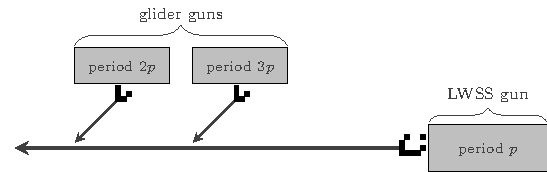
\includegraphics[width=0.95\textwidth]{periodic_circuitry/period_not_2_3_lwss_gun_schematic.pdf}
		\caption{A schematic for an LWSS gun that fires an irregular stream of spaceships with the property that the $n$-th spaceship in the stream is present if and only if $n$ is not a multiple of $2$ or $3$. Gliders are used to delete every second and every third spaceship in the LWSS stream.}
		\label{fig:period_not_2_3_lwss_gun_schematic}
	\end{minipage}
\end{figure}

To actually construct such a pattern, we make use of the period~$30$ circuitry that we have seen so far. If the period of the LWSS gun that we use is $p$, then we need glider guns with periods~$2p$ and~$3p$ as well. Since we do not yet know how to construct guns with periods~$60$ or~$90$ (we will learn how to do so in Section~\ref{sec:glider_deletion}), it seems natural to use the period~$120n$ guns based on the inline inverter that we introduced in Figure~\ref{fig:inline_inverter_p120_gun}. In particular, we arrange three period~$120$ guns so as to synthesize a lightweight spaceship, and then aim period~$240$ and~$360$ guns at the resulting LWSS stream in order to thin it out. The final pattern is displayed in Figure~\ref{fig:period_not_2_3_lwss_gun}.

\begin{figure}[!htb]
	\centering
	\patternimglink{0.1152}{period_not_2_3_lwss_gun}
	\caption{A gun that shoots an irregularly-spaced stream of lightweight spaceships. In particular, the period~$120$ inline inverter gun makes use of the glider-to-LWSS reaction from Figure~\ref{fig:glider_to_lwss} (highlighted in \bgbox{magentaback}{magenta}) to create a period~$120$ stream of lightweight spaceships (highlighted in \bgbox{greenpastel}{green}). Period~$240$ and period~$360$ inline inverter guns (highlighted in \bgbox{yellowback2}{yellow} and \bgbox{aquaback}{aqua}, respectively) then destroy every LWSS with a position in the stream that is a multiple of $2$ or $3$, respectively.}
	\label{fig:period_not_2_3_lwss_gun}
\end{figure}



\subsection{The Prime-Generating Gun Itself}\label{sec:primer_itself}

The gun that we just constructed contains the key idea used in our prime-generating gun---we create a period~$p = 120$ stream of lightweight spaceships and then aim glider guns with periods~$2p$, $3p$, $4p$, $5p$, and so on at the gun to delete any lightweight spaceships whose position in the stream is a multiple of $2$, $3$, $4$, $5$, $\ldots$, respectively.

The tricky part is that we now have to find a way to construct infinitely many glider guns (like the breeder) with ever-increasing periods (unlike the breeder). Fortunately, the period~$120n$ guns based on the inline inverter are perfect candidates for this task, since their periods are determined solely by how far apart the two Gosper glider guns at their ends are. Thus one way of constructing glider guns with ever-increasing periods is to send one set of rakes north to synthesize Gosper glider guns and another set of rakes east to do the same. The diagonal distance between these endpoint Gosper glider guns, along which a single glider will travel, increases without bound, giving us glider guns of larger and larger periods. We thus arrive at the schematic presented in Figure~\ref{fig:primer_schematic} for synthesizing these high-period glider guns and thus our primer.

\begin{figure}[!htb]
	\centering
	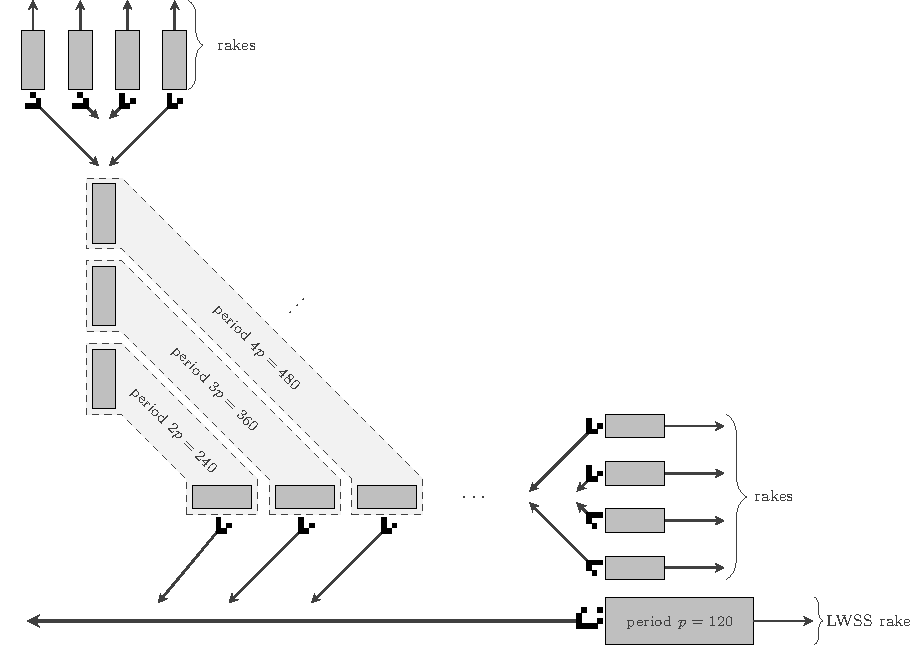
\includegraphics[width=\textwidth]{periodic_circuitry/primer_schematic.pdf}
	\caption{A schematic for a primer. For each integer $n \geq 2$, eastward and northward sets of rakes leave behind halves of the period~$120n$ glider gun based on the inline inverter, which is used to destroy every LWSS in the bottom period~$120$ stream whose position is a multiple of $n$. The only spaceships that escape to the far left are the ones whose position is not evenly divisible by any smaller integer $n \geq 2$ (i.e., the primes).}
	\label{fig:primer_schematic}
\end{figure}

This is by far our biggest construction to date---the breeder from Section~\ref{sec:gosper_breeder} was already quite large, and it just laid one row of Gosper glider guns, while this construction requires us to lay \emph{three} rows of Gosper glider guns (two going eastward and one going northward). It is thus worthwhile to present a more compact Gosper glider gun breeder that we can use as a component in our primer---see Figure~\ref{fig:breeder_compact}. Although this breeder looks quite different from our original one of the surface, it functions in more or less the same way by making use of several period~$60$ space rakes to gradually build the Gosper glider guns piece-by-piece.

\begin{figure}[!htb]
	\centering
	\embedlink{breeder_compact}{\vcenteredhbox{\patternimg{0.128}{breeder_compact}} \vcenteredhbox{\genarrow{360}} \vcenteredhbox{\patternimg{0.128}{breeder_compact_360}}}
	\caption{A compact breeder that uses $6$ period~$60$ space rakes to carry out an incremental synthesis of a Gosper glider gun. It gets away with fewer space rakes than our original breeder from Figure~\ref{fig:breeder_done} (which used $12$) since it cleverly manipulates the debris behind the two frontmost space rakes to create a ship, which is the most difficult part of the Gosper glider gun's incremental synthesis to create.}
	\label{fig:breeder_compact}
\end{figure}

Unfortunately, there are actually quite a few subtle problems with the previous schematic that prevent us from building it as-is:\smallskip

\begin{enumerate}
	\item[1)] The only Gosper glider gun breeders that we know how to build so far have period~$60$, which results in Gosper glider guns that are separated by $30$~cells, and thus inline inverter guns with periods that increase by $240$ (not $120$). In order to solve this problem, our first instinct might be to create a period~$240$ stream of lightweight spaceships instead of a period~$p = 120$ stream. However, we do not yet know how to do this.
	
	As an alternate solution, we use the breeders to create glider guns with periods~$3p$, $5p$, $7p$, $9p$, $\ldots$ (instead of $2p$, $3p$, $4p$, $5p$, $\ldots$) to delete any lightweight spaceships whose position in the stream is a multiple of $3$, $5$, $7$, $9$, $\ldots$, respectively. We then manually place a single glider gun of period~$2p$ to delete the leftover lightweight spaceships whose positions in the stream are a multiple of $2$.\smallskip
	
	\item[2)] With the Gosper glider guns just $30$~cells apart, we cannot fire gliders back and forth between them diagonally---the bouncing gliders would collide with the blocks that stabilize the glider guns.
	
	In order to solve this problem, we do the same thing that we did in Figure~\ref{fig:inline_inverter_p120_gun} to squeeze Gosper glider guns closer together---we replace one of the stabilizing blocks by an eater~1 (as in the buckaroo of Figure~\ref{fig:buckaroo_reflect}). To create a row of these modified Gosper glider guns, we can use the breeder displayed in Figure~\ref{fig:breeder_ggg_eater_1_stabilize}, which is just a slight modification of the breeders that we have already seen.\footnote{We already constructed a (much larger) breeder for this modification of the Gosper glider gun back in Exercise~\ref{exer:ggg_eater_side_breeder}.}\smallskip

	\begin{figure}[!htb]
		\centering
		\patternimglink{0.0984}{breeder_ggg_eater_1_stabilize}
		\captionof{figure}{A Gosper glider gun breeder that is stabilized on one side by an eater~1 instead of a block. The bottom half (highlighted in \bgbox{greenpastel}{green}) is the same as the bottom half of of the compact breeder from Figure~\ref{fig:breeder_compact}. The bottom-right space rake (highlighted in \bgbox{yellowback2}{yellow}) turns one of the blinkers from the blinker puffer (highlighted in \bgbox{magentaback}{magenta} and introduced in Exercise~\ref{exer:schick_engine_blinker_puffer}) into a ship via the incremental synthesis that we saw in Table~\ref{tab:sequential_synth}. The rightmost space rake (highlighted in \bgbox{orangeback2}{orange}) synthesizes the top ship into a queen bee, while the remaining three space rakes (highlighted in \bgbox{aquaback}{aqua}) synthesize the eater~1.}\label{fig:breeder_ggg_eater_1_stabilize}
	\end{figure}
	
	\item[3)] When the eastward breeders construct their two rows of Gosper glider guns, if their construction is not synchronized perfectly then the bottom row will release some gliders in the time between when it is constructed and when gliders from the top row are fed into it. This problem can be solved by using a fixed-length row of middleweight (or heavyweight) spaceships below those guns to destroy the excess gliders as in Figure~\ref{fig:orthogonal_destroy}.\smallskip
	
	\item[4)] A period $3p$ gun (for example) will erase all lightweight spaceships whose position in the stream is a multiple of $3$, \emph{including $3$ itself}, while we only want it to erase the multiples of $3$ greater than $3$. To solve this final problem, we can place a single block below each inline inverter gun in such a way that it destroys (and is destroyed by) the first glider released from the gun, thus preventing that first LWSS from being destroyed.\smallskip
\end{enumerate}

After putting all of these pieces together, we arrive at our completed primer in Figure~\ref{fig:primer}. We emphasize that static pictures really cannot do this pattern justice, so the reader is strongly encouraged to interact with and explore this pattern in Life-viewing software.\footnote{Like Golly: \httpurl{golly.sourceforge.net}.}

\begin{figure}[!htb]
	\centering
	\patternimglink{0.1115}{primer}
	\caption{The completed primer. The period~$120$ stream of lightweight spaceships (highlighted in \bgbox{orangeback2}{orange} and synthesized by $3$ space rakes as in Exercise~\ref{exer:p60_lwss_backrake}) moves to the left and is thinned out by the inline inverter guns (highlighted in \bgbox{aquaback}{aqua}). The leftmost inline inverter gun has period~$240$ and has a different shape from the others (which have periods~$360$, $600$, $840$, and in general $360 + 240n$ for $n \geq 0$). The rows of Gosper glider guns are laid by two copies of the compact breeder from Figure~\ref{fig:breeder_compact} (highlighted in \bgbox{greenpastel}{green}) and the row of Gosper glider guns that are stabilized by eater~1s instead of blocks are laid by the breeder that we presented in Figure~\ref{fig:breeder_ggg_eater_1_stabilize} (highlighted in \bgbox{yellowback2}{yellow}). A single space rake going north (also highlighted in \bgbox{yellowback2}{yellow}) produces the gliders that bounce along the long diagonal of the inline inverter guns, and the remaining pairs of space rakes (highlighted in \bgbox{magentaback}{magenta}) simply synthesize rows of block and eater~1s.}
	\label{fig:primer}
\end{figure}



\section{Period~46 Circuitry}\label{sec:p46}

Just like we can use the queen bee shuttle and Gosper glider gun as the basis of a set of period~$30$ circuitry, we can also use the twin bees shuttle (Figure~\ref{fig:twin_bees_shuttle}) and the related twin bees gun (Figure~\ref{fig:twin_bees_gun}) to build up a set of period~$46$ circuitry. For example, the twin bees shuttle can be used to reflect gliders and lightweight spaceships, and even convert gliders and lightweight spaceships \emph{into} each other, as displayed in Figure~\ref{fig:twin_bees_reflect}.\footnote{The 180~degree glider reflection takes 92~generations to complete, since the twin bees shuttle first converts the incoming glider into a block and then converts that block into the output glider. It was found by Dean Hickerson.}

We saw one of these glider reflections way back in Section~\ref{sec:sparkers}---the twin bees shuttle creates a duoplet spark\index{duoplet spark} that does the reflection.\footnote{This reflection is the one highlighted in green in Figure~\ref{fig:twin_bees_reflect_a}.} The other reflections and the glider-to-LWSS-to-glider conversions all make use of the large spark that is produced when one side of the twin bees shuttle is stabilized by just a single block.

\begin{figure}[!htb]
	\centering
	\begin{tabular}{@{}ccc@{}}
		\begin{subfigure}{.28\textwidth}
			\centering
			\embedlink{twin_bees_reflect}{\patternimg{0.09}{twin_bees_reflect_a}}
			\caption{three glider reflections}
			\label{fig:twin_bees_reflect_a}
		\end{subfigure} &
		\begin{subfigure}{.345\textwidth}
			\centering
			\embedlink{twin_bees_reflect}{\patternimg{0.09}{twin_bees_reflect_b}}
			\caption{two more reflections}
			\label{fig:twin_bees_reflect_b}
		\end{subfigure} &
		\begin{subfigure}{.325\textwidth}
			\centering
			\embedlink{twin_bees_reflect}{\patternimg{0.09}{twin_bees_reflect_c}}
			\caption{glider $\rightarrow$ LWSS and back}
			\label{fig:twin_bees_reflect_c}
		\end{subfigure}
	\end{tabular}
	\caption{The twin bees shuttle (highlighted in \bgbox{yellowback2}{yellow}) can be used to reflect a glider by 90~degrees in three different ways (highlighted in \bgbox{greenpastel}{green}), reflect a glider by 180~degrees (highlighted in \bgbox{aquaback}{aqua}), reflect a lightweight spaceship by 90~degrees (highlighted in \bgbox{magentaback}{magenta}), and turn a glider into a lightweight spaceship and back (highlighted in \bgbox{orangeback2}{orange}).}
	\label{fig:twin_bees_reflect}
\end{figure}

One of the advantages of these new reflections over the old reflection based on the duoplet spark is that they happen near the corner of the shuttle, so they can be used to (for example) merge two period~$46$ glider streams into a single period~$23$ stream, as in the period~$23$ glider gun displayed in Figure~\ref{fig:twin_bees_p23_gun}. Similarly, by making use of the glider-to-LWSS converter we can easily create period~$46$ LWSS guns without needing to synthesize them via three glider guns (see Figure~\ref{fig:twin_bees_p46_lwss_gun}). We can even use a careful arrangement of two twin bees shuttles to convert a lightweight spaceship into a middleweight one, and thus create small middleweight spaceship guns (see Figure~\ref{fig:twin_bees_lwss_to_mwss} and Exercise~\ref{exer:twin_bees_mwss_gun}). By replacing the input LWSS by an MWSS, this final LWSS-to-MWSS converter can also be used to simply reflect a MWSS by 90~degrees.%\footnote{We say that this is a \emph{pseudo}-period~$23$ gun since the gun itself operates at period~$46$. We discuss pseudo-period guns and true-period guns (which oscillate at the same period as the glider streams they produce) in depth in Chapter~\ref{chp:guns}.}

\begin{figure}[!htb]
	\centering
	\begin{tabular}{@{}ccc@{}}
		\begin{subfigure}{.37\textwidth}
			\centering
			\patternimglink{0.124}{twin_bees_p23_gun}
			\caption{a period~$23$ glider gun}
			\label{fig:twin_bees_p23_gun}
		\end{subfigure} & 
		\begin{subfigure}{.28\textwidth}
			\centering
			\patternimglink{0.13367804878}{twin_bees_p46_lwss_gun}
			\caption{a period~$46$ LWSS gun}
			\label{fig:twin_bees_p46_lwss_gun}
		\end{subfigure} & 
		\begin{subfigure}{.3\textwidth}
			\centering
			\patternimglink{0.13633830845}{twin_bees_lwss_to_mwss}
			\caption{LWSS $\rightarrow$ MWSS}
			\label{fig:twin_bees_lwss_to_mwss}
		\end{subfigure}
	\end{tabular}
	\caption{Various reflection and conversion reactions involving twin bees that can be used to create some useful guns. (a) is a period~$23$ glider gun constructed by reflecting one period~$46$ stream into the gaps in another period~$46$ stream, (b) is a lightweight spaceship gun that uses the glider-to-LWSS conversion from Figure~\ref{fig:twin_bees_reflect_c}, and (c) is an LWSS-to-MWSS conversion that (for example) allows for the construction of a small MWSS gun.}
	\label{fig:twin_bees_weird_guns}
\end{figure}

There are also a few other useful reactions involving the twin bees that can do things like emit two side-by-side streams of gliders (guns like this are called \emph{double-barreled guns}\index{double-barreled gun}). We explore some of these reactions in Exercise~\ref{exer:twin_bees_large_spark}.


%%%%%%%%%%%%%%%%%%%%%%%%%%%%%%%%%%%%%%%%%%%%%%%%%%%%%%%%%%%%%%%%%%%%%%%%%
%%   SUBSECTION: TICKER TAPES and MEMORY CELLS
%%%%%%%%%%%%%%%%%%%%%%%%%%%%%%%%%%%%%%%%%%%%%%%%%%%%%%%%%%%%%%%%%%%%%%%%%
\subsection{Ticker Tapes and Memory Cells}\label{sec:p46_ticker_tape}

One of the most useful reactions involving a twin bees shuttle that we have not yet seen is the one displayed in Figure~\ref{fig:twin_bees_duplicate_reflector} in which the shuttle reflects a glider by $90$~degrees while simultaneously duplicating it (similar to the p$30$ glider duplicator that we saw in Figure~\ref{fig:periodic_glider_duplicator}).

One interesting thing that we can do with a glider duplicator is attach it to a glider loop so as to produce any (finite) irregular sequence of gliders of our choosing, simply by having that sequence of gliders in the loop itself. For example, the pattern displayed in Figure~\ref{fig:ticker_tape_gun} makes use of a loop in which one glider is present, then the next two are missing, then the next three are present, then four are missing, five are present, and six are missing, so as to create a gun that produces lightweight spaceships with that same spacing.\footnote{This gun produces lightweight spaceships (via the glider-to-LWSS reaction of Figure~\ref{fig:twin_bees_reflect_c}) instead of gliders just to make the output easier to visualize.} We can thus encode any message in binary and create a gun that emits that message if we interpret the presence of a spaceship as a ``1'' and the absence of a spaceship as a ``0''.

\begin{figure}[!htb]
	\centering
	\begin{tabular}{@{}cc@{}}
		\begin{minipage}[t]{0.208\textwidth}
			\centering
			\patternimg{0.15830666666}{twin_bees_duplicate_reflector}
			\caption{A twin bees shuttle reflecting and duplicating a glider.}\label{fig:twin_bees_duplicate_reflector}
		\end{minipage} &
		\begin{minipage}[t]{0.762\textwidth}
			\centering
			\patternimglink{0.093}{ticker_tape_gun}
			\caption{A gun that produces an irregular lightweight spaceship stream corresponding to the bitstring 100111000011111000000 (i.e., one LWSS present, then two missing, then three present, and so on). This stream (highlighted in \bgbox{orangeback2}{orange}) is produced by duplicating the gliders in the loop (highlighted in \bgbox{aquaback}{aqua}) that have this same spacing and then performing a few reflections and a glider-to-LWSS conversion via twin bees shuttles (highlighted in \bgbox{yellowback2}{yellow}).}\label{fig:ticker_tape_gun}
		\end{minipage}
	\end{tabular}
\end{figure}

By placing several of these guns near each other (with different sequences of gliders in their glider loops), we can even create \emph{ticker tape guns}\index{ticker tape gun}, which emit any \emph{visual} message of our choosing, rather than just messages encoded in binary. To do this, we think of lightweight spaceships as pixels, with the presence of a ship being black and the absence of a ship being white. Each of the loop-based guns emits the pixels (ships) in a single row of the image being produced, so we use $n$ of the guns with $m$ gliders each in the loops to create an $n \times m$ image. For example, Figure~\ref{fig:ticker_tape_hi_gun} illustrates a ticker tape gun that repeatedly produces an $8 \times 21$ array of lightweight spaceships that spells out ``HI!''.\footnote{Alan Hensel put together the first ticker tape gun in June 1994, which printed out the digits ``0123456789''. It was adapted by Brice Due and Dave Greene in 2005 and 2006 to print out the Golly logo, and has been used as the header of the Golly homepage (\httpurl{golly.sourceforge.net/}) ever since.}

\begin{figure}[!htb]
	\centering
	\patternimglink{0.0985}{ticker_tape_hi_gun}
	\caption{An arrangement of $8$ loop-based guns that produce an array of lightweight spaceships that spell out ``HI!'' (highlighted in \bgbox{orangeback2}{orange}). Each gun produces one row of the output image (highlighted in \bgbox{yellowback2}{yellow}, \bgbox{magentaback}{magenta}, \bgbox{greenpastel}{green}, and \bgbox{aquaback}{aqua}), and the arrangement of gliders in each loop determines which lightweight spaceships are produced in their row.}\label{fig:ticker_tape_hi_gun}
\end{figure}

Once we start talking about building things like computers in the Game of Life (which we will do in Chapter~\ref{chp:universal_computation}), loops like this will be quite useful since they can serve as pieces of memory for the computer to make use of (for example, the gun in Figure~\ref{fig:ticker_tape_gun} stores the bitstring ``100111000011111000000'', which we can read from memory by detecting the spaceships that are constantly emitted from the gun). To make loops like this truly useful for storing pieces of information though, we need to be able to easily alter the state of the memory (i.e., delete gliders from the loop and also insert new gliders into it).

Deleting a glider from the loop is simple, since we can just fire another glider from elsewhere in the Life plane so as to collide with it, thus deleting them both. To turn this deletion operation into an \emph{insertion} operation, we can simply place two stream inverters along the loop and apply the deletion operation somewhere along its inverted portion. A pattern that makes use of these ideas is called a \emph{memory cell}\index{memory cell}, and one is illustrated in Figure~\ref{fig:p46_memory_cell} along with the mechanisms for altering the contents of its memory.

\begin{figure}[!htb]
	\centering
	\embedlink{p46_memory_cell}{\vcenteredhbox{\patternimg{0.108}{p46_memory_cell_0}} \vcenteredhbox{\genarrow{552}} \vcenteredhbox{\patternimg{0.108}{p46_memory_cell_552}}}
	\caption{A period $12 \times 46 = 552$ memory cell for which the $12$-bit string ``111010111011'' is encoded along its glider loop (highlighted in \bgbox{aquaback}{aqua}) and is thus repeatedly fired out as a stream of lightweight spaceships (highlighted in \bgbox{orangeback2}{orange}). Bits can be switched from $1$ to $0$ (i.e., gliders can be deleted) by sending in a glider from the northwest (highlighted in \bgbox{magentaback}{magenta}) to collide with the loop. Since the northeast side of the glider loop is inverted, bits can be switched from $0$ to $1$ (i.e., gliders can be inserted) by similarly sending in a glider from the northeast (highlighted in \bgbox{greenpastel}{green}) to collide with that side of the loop. As shown here, the $8$th and $10$th bits are flipped, thus changing the bitstring in memory to ``1110101\textbf{0}1\textbf{1}11''.}\label{fig:p46_memory_cell}
\end{figure}


%%%%%%%%%%%%%%%%%%%%%%%%%%%%%%%%%%%%%%%%%%%%%%%%%%%%%%%%%%%%%%%%%%%%%%%%%
%%   SUBSECTION: TANNER'S P46
%%%%%%%%%%%%%%%%%%%%%%%%%%%%%%%%%%%%%%%%%%%%%%%%%%%%%%%%%%%%%%%%%%%%%%%%%
\subsection{Tanner's p46}\label{sec:p46_tanner}

One of the most useful tools for extending our period~$46$ toolset beyond just things that can be done with twin bees is the extremely sparky period~$46$ oscillator called \emph{Tanner's p46}\index{Tanner's p46} that we saw back in Figure~\ref{fig:tanners_p46}. As is typical of extremely sparky oscillators, Tanner's p46 can be combined with other sparkers, or additional copies of itself, to create numerous useful objects. For example, it can be combined with a twin bees shuttle to create a new p$46$ glider gun (see Exercise~\ref{exer:tanners_p46_twin_bee_gun}), or it can be used to reflect a glider by 180~degrees (see Exercise~\ref{exer:tanners_p46_reflect}), but neither of these facts are too exciting since we already know how to construct p$46$ glider guns and reflectors of roughly the same size via twin bees.

What is slightly more interesting is that we can carefully place two copies of Tanner's p46 next to each other so as to construct an \emph{edge-shooting glider gun},\footnote{Found by David Bell just three days after Tanner's p$46$ itself was found.}\index{edge shooter} as illustrated in Figure~\ref{fig:tanners_p46_edge}. Edge shooters like this one are particularly useful when trying to line up streams of gliders in tight positions, since they can be positioned as close as we like to existing glider streams on one side (compare this with guns like the Gosper glider gun and twin bees guns, which produce the stream of gliders near their center and thus require some clearance on either side of the other glider stream).

Furthermore, this glider gun can act as a p$46$ inline inverter (see Figure~\ref{fig:tanners_p46_inline_inverter}) just like the Gosper glider gun can act as a p$30$ inline inverter.\footnote{This inline inverter, just like the original p$30$ one, was found by David Bell.} Even more remarkably, two of these oscillators can be placed next to each other so as to create the p$46$ middleweight spaceship gun displayed in Figure~\ref{fig:tanners_p46_mwss_gun},\footnote{Found by Matthias Merzenich just one day after Tanner's p$46$ was found.} which is currently the smallest known MWSS gun of any period, and also the smallest known gliderless gun of any period.

\begin{figure}[!htb]
	\centering
	\begin{tabular}{@{}ccc@{}}
		\begin{subfigure}{.355\textwidth}
			\centering
			\patternimglink{0.10424012158}{tanners_p46_edge}
			\caption{an edge-shooting glider gun}
			\label{fig:tanners_p46_edge}
		\end{subfigure} &
		\begin{subfigure}{.345\textwidth}
			\centering
			\patternimglink{0.095}{tanners_p46_inline_inverter}
			\caption{an inline inverter}
			\label{fig:tanners_p46_inline_inverter}
		\end{subfigure} &
		\begin{subfigure}{.24\textwidth}
			\centering
			\patternimglink{0.0971529745}{tanners_p46_mwss_gun}
			\caption{a small MWSS gun}
			\label{fig:tanners_p46_mwss_gun}
		\end{subfigure}	
	\end{tabular}
	\caption{Two guns formed by placing two copies of Tanner's p$46$ next to each other so that their sparks interact. The glider gun from (a) can be used as an inline inverter, as in (b), where the incoming glider (highlighted in \bgbox{greenpastel}{green}) prevents a glider from being fired from the gun at that point in the stream. The gun in (c) is the smallest known MWSS gun.}
	\label{fig:tanners_p46_guns}
\end{figure}

As an example of what can be done with the edge-shooting gun of Figure~\ref{fig:tanners_p46_edge}, we note that it can be used to make a heavyweight spaceship gun via the $3$-glider HWSS synthesis that we saw back in Table~\ref{tab:3_glider_synth}, even though this synthesis contains closely-spaced gliders that cannot be placed by the ``usual'' guns that we have seen so far. An example of such a gun is presented in Figure~\ref{fig:p46_hwss_gun}.

\begin{figure}[!htb]
	\centering
	\patternimglink{0.08}{p46_hwss_gun}
	\caption{A period~$46$ heavyweight spaceship gun that uses two copies of the edge shooter from Figure~\ref{fig:tanners_p46_edge} (highlighted in \bgbox{aquaback}{aqua} and \bgbox{magentaback}{magenta}) to place the required gliders in the HWSS synthesis close together.}
	\label{fig:p46_hwss_gun}
\end{figure}


%%%%%%%%%%%%%%%%%%%%%%%%%%%%%%%%%%%%%%%%%%%%%%%%%%%%%%%%%%%%%%%%%%%%%%%%%
%%   SUBSECTION: HEISENBURPS
%%%%%%%%%%%%%%%%%%%%%%%%%%%%%%%%%%%%%%%%%%%%%%%%%%%%%%%%%%%%%%%%%%%%%%%%%
\subsection{Heisenburps}\label{sec:p46_heisenburps}

We saw back in Figure~\ref{fig:periodic_glider_duplicator} that it is possible to construct periodic circuits that duplicate gliders, though the timing and positioning of the output gliders typically do not match those of the input glider.\footnote{In fact, we saw that there are \emph{stationary} circuits that duplicate gliders way back in Figure~\ref{fig:894_reflector}, but these circuits will remain a bit more mysterious until Chapter~\ref{chp:stationary_circuitry}.} We could of course use various other circuits to correct the positioning and timing of one of the output gliders, but remarkably there exist duplicators for which this is not necessary, as the input glider is not actually affected at all (even temporarily) by the duplication process.

Duplicators of this type are called \emph{Heisenburps}\index{Heisenburp}\footnote{Named for Heisenberg's uncertainty principle, which says that it is impossible to detect a particle without affecting it in some way. Heisenburps show that this principle does \emph{not} hold in Conway's Game of Life, since we can detect and duplicate a particle (glider) without affecting it at all.}, and by far the simplest one known is displayed in Figure~\ref{fig:p46_natural_heisenburp}.\footnote{Found by Brice Due in January 2005.} In this configuration, the spark from two perpendicular twin bees is suppressed slightly by a passing glider so that instead of dying off, the spark turns into another glider. Importantly, the passing glider itself is not affected at all in the process, but rather just serves to overpopulate other nearby cells (much like how we used induction coils to overpopulate and stabilize objects in Section~\ref{sec:still_life_grammar}).

\begin{figure}[!htb]
	\centering
	\embedlink{p46_natural_heisenburp}{\vcenteredhbox{\patternimg{0.133}{p46_natural_heisenburp_0}} \vcenteredhbox{\genarrow{46}} \vcenteredhbox{\patternimg{0.133}{p46_natural_heisenburp_46}} \vcenteredhbox{\genarrow{46}} \vcenteredhbox{\patternimg{0.133}{p46_natural_heisenburp_92}}}
	\caption{A small period~$92$ Heisenburp that uses two twin bees shuttles (highlighted in \bgbox{yellowback2}{yellow}) to copy a glider (highlighted in \bgbox{greenpastel}{green}) without affecting it. The first $46$ generations are used to create a block (highlighted in \bgbox{orangeback2}{orange}) from the glider, and the next $46$ generations are used to turn the block into another glider.}\label{fig:p46_natural_heisenburp}
\end{figure}

There are also Heisenburps that can copy other spaceships, or even use one type of passing spaceship to create a completely different kind of object---all that is needed is a spark whose evolution is changed sufficiently by the passing spaceship that it turns into something that moves out of the way. For example, the configuration of two twin bees shuttles in Figure~\ref{fig:mwss_out_of_the_blue}, called the \emph{MWSS out of the blue}\index{MWSS out of the blue},\footnote{Found by Peter Rott in November 1997.} detects a passing lightweight spaceship and releases a middleweight spaceship travelling in the opposite direction in response.

\begin{figure}[!htb]
	\centering
	\embedlink{mwss_out_of_the_blue}{\vcenteredhbox{\patternimg{0.11}{mwss_out_of_the_blue_0}} \vcenteredhbox{\genarrow{46}} \vcenteredhbox{\patternimg{0.11}{mwss_out_of_the_blue_46}}}
	\caption{The \emph{MWSS out of the blue} is a reaction in which two twin bees shuttles are triggered to create a middleweight spaceship when a lightweight spaceship passes by. The LWSS is not affected at all by the reaction.}\label{fig:mwss_out_of_the_blue}
\end{figure}

There are also some reactions that can be used to construct Heisenburps via other periodic circuitry that we have already seen. One of the simplest such reactions is the one displayed in Figure~\ref{fig:heisenburp_reaction_p35},\footnote{Found by Jason Summers in June 1999, as was the first-known period~$46$ Heisenburp based on it.} in which a middleweight and heavyweight spaceship collide with a glider in such a way that if another passing glider is present, then the three colliding spaceships cleanly destroy each other, but if that passing glider is absent then they produce a single glider. This reaction has a repeat time of $35$~generations and thus can be used to construct Heisenburps of any period~$35$ or greater.

\begin{figure}[!htb]
	\centering
	\begin{subfigure}{.47\textwidth}
		\centering
		\embedlink{heisenburp_reaction_p35}{\vcenteredhbox{\patternimg{0.12}{heisenburp_reaction_p35_0_0}} \vcenteredhbox{\genarrow{19}} \vcenteredhbox{\patternimg{0.12}{heisenburp_reaction_p35_0_19}}}
		\caption{Mutual annihilation if a nearby glider is present.}
		\label{fig:heisenburp_reaction_p35_0}
	\end{subfigure} \ \ \ \ % 
	\begin{subfigure}{.5\textwidth}
		\centering
		\embedlink{heisenburp_reaction_p35}{\vcenteredhbox{\patternimg{0.12}{heisenburp_reaction_p35_1_0}} \vcenteredhbox{\genarrow{19}} \vcenteredhbox{\patternimg{0.12}{heisenburp_reaction_p35_1_19}}}
		\caption{Production of a glider if no nearby glider is present.}
		\label{fig:heisenburp_reaction_p35_1}
	\end{subfigure}
	\caption{A collision of a glider, lightweight spaceship, and heavyweight spaceship (highlighted in \bgbox{yellowback2}{yellow}) that results in (a) nothing if there is a nearby passing glider (highlighted in \bgbox{greenpastel}{green}), and (b) a single glider (highlighted in \bgbox{orangeback2}{orange}) if there is not a nearby passing glider. Since the passing glider is unaffected by the collision, this reaction can be used as a basis for a Heisenburp.}\label{fig:heisenburp_reaction_p35}
\end{figure}

To actually construct a Heisenburp from this reaction, we just combine reactions that we saw earlier---we know how to create streams of gliders, middleweight spaceships, and heavyweight spaceships, so we have no problem creating the three objects needed to fuel the reaction, and then we can just use the stream inverter of our choice to ``fix'' the duplicated output stream (since the reaction creates a glider if and only if an input glider is \emph{not} present, which is the opposite of what we want). Figure~\ref{fig:p46_heisenburp_constructed} demonstrates one way to put these pieces together using period~$46$ circuitry, but any set of sufficiently-high period circuits work.

\begin{figure}[!htb]
	\centering
	\embedlink{p46_heisenburp_constructed}{\vcenteredhbox{\patternimg{0.088}{p46_heisenburp_constructed}} \vcenteredhbox{\genarrow{230}} \vcenteredhbox{\patternimg{0.088}{p46_heisenburp_constructed_230}}}
	\caption{A period~$46$ Heisenburp that uses the glider $+$ MWSS $+$ HWSS reaction from Figure~\ref{fig:heisenburp_reaction_p35}. These spaceships are all provided by guns that we have already seen---the MWSS gun (highlighted in \bgbox{aquaback}{aqua}) and HWSS gun (highlighted in \bgbox{magentaback}{magenta}) were introduced in Figures~\ref{fig:tanners_p46_mwss_gun} and~\ref{fig:p46_hwss_gun}, respectively. The central three-spaceship collision produces a (non-highlighted) glider traveling northeast, which is destroyed by an inline inverter (highlighted in \bgbox{orangeback2}{orange} and originally introduced in Figure~\ref{fig:tanners_p46_inline_inverter}). However, if an input glider (highlighted in \bgbox{greenpastel}{green}) is present then no glider is fed into the inline inverter, leading to the input glider's duplication.}\label{fig:p46_heisenburp_constructed}
\end{figure}

In fact, we can use these same ideas to even construct \emph{stationary} Heisenburps (i.e., Heisenburps made up entirely of still lifes, rather than oscillators and guns), as long as the spaceship that is being detected and duplicated has an accessible spark, like an xWSS. However, a glider Heisenburp must have an oscillating component, as gliders have no accessible sparks that could be detected by still lifes.


\section{Bumpers and Bouncers}\label{sec:bumper_bouncer}

Some periodic circuitry works based only on the existence of certain sparks, and thus can be made to work at any period for which we know of oscillators that emit that spark. For example, the glider-reflecting reactions of Figure~\ref{fig:spark_glider_reflect} fall into this category, since any oscillator that produces the correct banana spark (such as a buckaroo) or duoplet spark (such as the twin bees shuttle) can be used to implement the reflection. However, most of the oscillators that emit these sparks have rather large period, so we now introduce two other spark-based glider reflectors that can make use of low-period oscillators.

The first of these reactions is called the \emph{bumper}\index{bumper} (displayed in Figure~\ref{fig:bumper}),\footnote{The p$3$ bumper was found in April 2018 by Arie Paap, but the reaction itself and most of the other bumpers were found in April 2016 by Tanner Jacobi.} which consists of an eater~1, a loaf, and a spark\index{spark} of almost any type. This reflector is versatile enough that it can be used with a wide variety of sparkers, including some with period as low as~$3$ (see Figure~\ref{fig:bumper} for numerous examples). Since this reflector is color-preserving\index{glider!color}, just like the Snark, it perhaps does not seem too exciting at first glance (after all, stable reflectors work at \emph{any} period). However, there are at least three reasons why bumpers are still useful:\smallskip

\begin{figure}[!htb]
	\centering
	\begin{tabular}{@{}ccc@{}}
		\begin{subfigure}{.29\textwidth}
			\centering\vspace*{0.15cm}
			\patternimglink{0.145}{bumper}
			\caption{The bumper itself. A spark must be present at the location marked in \bgbox{redback}{red} $11$~generations after the input glider's phase shown here.}
			\label{fig:bumper_raw}
		\end{subfigure} &
		\begin{subfigure}{.29\textwidth}
			\centering\vspace*{-0.85cm}
			\patternimglink{0.124408284}{p3_bumper_b}
			\caption{A p$3$ bumper that uses a custom oscillator.}
			\label{fig:p3_bumper_a}
		\end{subfigure} &
		\begin{subfigure}{.34\textwidth}
			\centering\vspace*{-0.85cm}
			\patternimglink{0.145}{p3_bumper_a}
			\caption{Another p$3$ bumper that uses a custom oscillator.}
			\label{fig:p3_bumper_b}
		\end{subfigure} \\[2.7cm]
		\begin{subfigure}{.29\textwidth}
			\centering
			\patternimglink{0.12}{p4_bumper}
			\caption{A p$4$ bumper that uses a custom oscillator.}
			\label{fig:p4_bumper}
		\end{subfigure} &
		\begin{subfigure}{.29\textwidth}
			\centering
			\patternimglink{0.12596273291}{p6_bumper}
			\caption{A p$6$ bumper reflector that uses the unix sparker.\index{unix}}
			\label{fig:p6_bumper}
		\end{subfigure} &
		\begin{subfigure}{.34\textwidth}
			\centering
			\patternimglink{0.13986206896}{p7_bumper}
			\caption[p7 bumper]{A p$7$ bumper that uses Beluchenko's p7 from Figure~\ref{fig:sparky_p7}.}
			\label{fig:p7_bumper}
		\end{subfigure} \\[2cm]
		\begin{subfigure}{.29\textwidth}
			\centering\vspace*{0.1cm}
			\patternimglink{0.13}{p8_bumper}
			\caption{A p$8$ bumper reflector that uses the blocker\index{blocker}.}
			\label{fig:p8_bumper}
		\end{subfigure} &
		\begin{subfigure}{.29\textwidth}
			\centering\vspace*{0.1cm}
			\patternimglink{0.13}{p9_bumper}
			\caption{A p$9$ bumper reflector that uses the p$9$ thumb sparker\index{thumb spark}.}
			\label{fig:p9_bumper}
		\end{subfigure} &
		\begin{subfigure}{.34\textwidth}
			\centering
			\patternimglink{0.10124423963}{p11_bumper}
			\caption{A p$11$ bumper reflector that uses a custom oscillator.}
			\label{fig:p11_bumper}
		\end{subfigure}
	\end{tabular}
	\caption{The bumper is a glider reflector that relies on a single spark. Because the spark is somewhat distant from the reflection reaction itself, it can be provided by a wide variety of different oscillators (outlined in \bgbox{aquaback}{aqua}) and can thus work with many different periods. Note that the period~$4$ and~$11$ bumpers use a slightly different spark based on hassling a block. Some bumpers of other periods (including a very useful p$5$ bumper) are explored in Exercise~\ref{exer:bumper_high_period}.}
	\label{fig:bumper}
\end{figure}

\begin{enumerate}
	\item[1)] It is smaller (and, for many periods, easier to synthesize) than the Snark.\smallskip
	
	\item[2)] The Snark has a repeat time of $43$~generations, whereas the bumper has a repeat time of just $34$~generations. However, the input glider stream must be compatible with the period of the oscillator, so for example the p$3$, p$4$, and p$6$ bumpers actually have repeat time $36$, and the p$5$ and p$7$ bumpers actually have repeat time $35$.\smallskip
	
	\item[3)] Its reflected gliders have different timing than those reflected by the Snark. Specifically, a bumper produces a glider that has timing\index{glider!timing} exactly $5$~generations delayed from that of a glider reflected by a Snark. This is a useful feature when fine-tuning the positioning of gliders along glider tracks, as we can replace Snarks by bumpers to rephase the gliders (similar to how we used a wide variety of different one-time reflectors in Table~\ref{tab:180_degree_one_time_turners} to get precise glider timings).\smallskip
\end{enumerate}

There is another closely-related reaction called the \emph{bouncer}\index{bouncer} (displayed in Figure~\ref{fig:bouncer_reflector}),\footnote{The bouncer, as well as most of the low-period pipsquirters that it can use, were found by Noam Elkies in September 1998.} which consists of an eater~1, a boat, a block, and a domino spark that is typically provided by a pipsquirter\index{pipsquirter}. The bouncer is somewhat less versatile than the bumper since the domino spark is tricky to position correctly, but it also has the advantage of having a repeat time of just $22$~generations (versus the bumper's $34$ and the Snark's $43$). Furthermore, these reflectors are color-changing,\footnote{Their names are designed to help us remember which reaction is color-preserving and which one is color-changing---the bum\textbf{p}er is color-\textbf{p}reserving while the boun\textbf{c}er is color-\textbf{c}hanging.} which provides us with some extra flexibility that we did not yet have (recall that both the Snark and the bumper are color-preserving).\footnote{For a more complete and up-to-date collection of bumpers and bouncers, see \httpsurl{conwaylife.com/wiki/Bumper_and_bouncer_gallery}.}

\begin{figure}[!htb]
	\centering
	\begin{tabular}{@{}ccc@{}}
		\begin{subfigure}{.29\textwidth}
			\centering\vspace*{0.2cm}
			\patternimg{0.15}{pipsquirter_raw_reflect}
			\caption{The bouncer itself. A spark must be present at the \bgbox{redback}{red} location, or one cell farther south, $14$~generations after the input glider's phase shown here.}
			\label{fig:pipsquirter_raw_reflect}
		\end{subfigure} &
		\begin{subfigure}{.33\textwidth}
			\centering\vspace*{-1.1cm}
			\patternimglink{0.13431372549}{p6_bouncer}
			\caption{A p$6$ bouncer.}
			\label{fig:p6_bouncer}
		\end{subfigure} &
		\begin{subfigure}{.32\textwidth}
			\centering\vspace*{-1.1cm}
			\patternimglink{0.08526970954}{p7_bouncer}
			\caption{A p$7$ bouncer.}
			\label{fig:p7_bouncer}
		\end{subfigure} \\[2.6cm]
		\begin{subfigure}{.29\textwidth}
			\centering
			\patternimglink{0.11418918918}{p8_bouncer}
			\caption{A p$8$ bouncer that uses a figure eight\index{figure eight}.}
			\label{fig:p8_bouncer}
		\end{subfigure} &
		\begin{subfigure}{.33\textwidth}
			\centering
			\patternimglink{0.125}{p15_bouncer}
			\caption{A p$15$ bouncer based on an oscillator called \emph{Karel's p15}\index{Karel's p15}.}
			\label{fig:p15_bouncer}
		\end{subfigure} &
		\begin{subfigure}{.32\textwidth}
			\centering
			\patternimglink{0.07738095238}{p5_bouncer}
			\caption{A closely-related p$5$ reflector that uses a dot sparker.}
			\label{fig:p5_bouncer}
		\end{subfigure}
	\end{tabular}
	\caption{Pipsquirters (as well as a handful of other domino sparkers) can be used to with the bouncer to reflect gliders. This allows for the creation of several new reflectors with many periods.}
	\label{fig:bouncer_reflector}
\end{figure}

%While this family of reflectors only works directly with period of $6$ and greater, a very similar reaction can be made to work at period~$5$, thus giving us our very first period~$5$ reflector in Figure~\ref{fig:p5_bouncer}. For a period~$5$ reflector based on the bumper, see Exercise~\ref{exer:bumper_high_period}.


\section{Glider Timing and Regulators}\label{sec:periodic_regulators}

Oftentimes when trying to construct a large pattern, we know there will be a signal coming in from somewhere else in a mechanism---usually a glider arriving on some particular path. Once this input comes in, we want to perform a specific action, but it should only occur on a specific schedule, so as to be compatible with some set of circuitry. For example, we might want to send out a glider to be reflected back by a receding spaceship that has a known speed and position, but if the timing isn't exactly right then the reflection reaction won't work.

To illustrate how we can overcome this problem, suppose for now that we have a glider at some specific location, and we need to relocate it so that it appears at another pre-specified location with a certain timing. If the input glider is on some kind of schedule---say, it only has a possibility of showing up once every $30$~ticks, or more generally once every $n$~ticks for any reasonably high value of $n$---then this job is easy. We just line up a period~$n$ gun with an inverter of the same period, and then find a way for the arriving glider to cleanly delete a glider from the stream that hits the inverter. The inverter then sends out a glider in response to the resulting hole in the stream, thus producing an output glider at the desired location and timing.

The only somewhat tricky part here is getting the input glider to cleanly destroy a single glider in the stream that will be inverted, since we do not have control over the inverter's position or timing (they are determined by where and when we want the output glider to appear). However, we can change the positioning and timing of the input glider in a variety of ways, the simplest of which is to add some additional reflectors to the input glider's path (see Figure~\ref{fig:inverter_as_regulator}). Some trial-and-error is required here to produce a configuration of reflectors that results in the desired clean glider annihilation, but sooner rather than later, along the same lines as Exercises~\ref{exer:glider_cleanup}--\ref{exer:glider_block_collisions}, a workable two-glider collision will be found. As shown in Table~\ref{tab:2_glider_synth}, there are a lot of options that result in clean mutual annihilation---as long as we can make adjustments to change the collision timing, the odds are heavily in our favor that we will find one.

\begin{figure}[!htb]
	\centering
	\begin{subfigure}{.49\textwidth}
		\centering
		\embedlink{inverter_as_regulator_0}{\vcenteredhbox{\patternimg{0.086}{inverter_as_regulator_0_0}} \vcenteredhbox{\genarrow{120}} \vcenteredhbox{\patternimg{0.086}{inverter_as_regulator_0_120}}}
		\caption{A glider (unfortunately) destroying $3$ gliders.}
		\label{fig:inverter_as_regulator_0}
	\end{subfigure} \ \ \ % 
	\begin{subfigure}{.48\textwidth}
		\centering
		\embedlink{inverter_as_regulator_1}{\vcenteredhbox{\patternimg{0.086}{inverter_as_regulator_1_0}} \vcenteredhbox{\genarrow{120}} \vcenteredhbox{\patternimg{0.086}{inverter_as_regulator_1_120}}}
		\caption{Once re-timed, just one glider is destroyed.}
		\label{fig:inverter_as_regulator_1}
	\end{subfigure}
	\caption{An input glider (highlighted in \bgbox{greenpastel}{green}) being re-timed to fit with existing p$30$ circuitry by a Gosper glider gun firing into an inline inverter (highlighted in \bgbox{yellowback2}{yellow}). As positioned in (a), the input glider destroys three of the gliders in the stream, so three gliders are released to the northeast. We can correct this problem by using two buckaroos (highlighted in \bgbox{aquaback}{aqua} in (b)) to reflect the glider twice and thus change the timing with which it hits the glider streem between the two Gosper glider guns. After some trial-and-error, we find the configuration in (b) where just a single glider is destroyed.}\label{fig:inverter_as_regulator}
\end{figure}

What if $n$ (the period to which the input and output gliders are aligned) is low enough that we can't build a period~$n$ gun? For example, suppose that all we know about the input stream of gliders is that they are separated by generation gaps that are multiples of~$8$. We cannot build a period~$8$ gun to aim at an inline inverter (recall that the lowest-period glider stream possible is period~$14$), but we could instead reflect the glider with Snarks and period~$8$ bouncers and bumpers, which can be used to produce any possible output lane and sufficiently slow timing.

What if we go one step further and suppose that we do not know \emph{anything at all} about the input glider's timing, but we still want to be able to insert it into periodic circuitry (i.e., we want to align that glider to some specific period)? Unfortunately, neither of the previously-mentioned techniques work in this scenario:\smallskip

\begin{itemize}
	\item We cannot simply have the input glider interrupt a stream from a glider gun as in Figure~\ref{fig:inverter_as_regulator}. That method will work for some timings, but other timings will result in multiple gliders being deleted or even chaotic explosions.\smallskip
	
	\item We cannot simply reflect the input gliders to get whatever timing we want, as we can only arrange reflectors so as to get the first glider on the input stream to have the correct timing---not subsequent gliders (e.g., if two gliders come in along the input stream with a separation of $58$ gliders, there is no way to use just Snarks so as to widen that gap to $60$ generations).\smallskip
\end{itemize}

What we need instead is a reaction that always works the same way, producing an output glider aligned to a particular period, no matter what the precise timing of the input glider is (as long as the separation between consecutive input gliders is no smaller than the output period). A mechanism that accomplishes this for a particular output period is called a \emph{regulator}\index{regulator}, and a mechanism that can be adjusted to work at any period is known as a \emph{universal regulator}\index{universal regulator}.


\subsection{A Universal Regulator}\label{sec:chapman_universal_regulator}

We now describe how the first universal regulator was built.\footnote{By Paul Chapman in March 2003.} The heart of this regulator is actually the boat bit\index{boat!bit} from way back in Section~\ref{sec:rocks_almost_eaters}, which is displayed again in Figure~\ref{fig:boat_bit_ch6}. In particular, if we use an eater~1 (instead of a snake as in Figure~\ref{fig:boat_bit}), then a duoplet spark can be used to test whether or not the boat bit is present (i.e., whether or not the input glider has arrived yet). In particular, the duoplet spark does not come close enough to the eater~1 to affect it, but if the boat bit is present then the boat and eater are both destroyed, producing an output glider as in Figure~\ref{fig:boat_bit_into_glider}. A beehive is also created, but this can easily be destroyed later.

\begin{figure}[!htb]
	\centering
	\begin{tabular}{@{}cc@{}}
		\begin{minipage}[t]{0.515\textwidth}
			\centering
			\embedlink{boat_bit}{\vcenteredhbox{\patternimg{0.1}{boat_bit_0}} \vcenteredhbox{\genarrow{12}} \vcenteredhbox{\patternimg{0.1}{boat_bit_12}} \vcenteredhbox{\genarrow{8}} \vcenteredhbox{\patternimg{0.1}{boat_bit_20}}}
			\caption{A boat-bit using an eater~1. The first input glider creates a boat, and the second destroys it.}\label{fig:boat_bit_ch6}
		\end{minipage} &
		\begin{minipage}[t]{0.455\textwidth}
			\centering
			\embedlink{boat_bit_into_glider}{\vcenteredhbox{\patternimg{0.096330275229}{boat_bit_into_glider_0}} \vcenteredhbox{\genarrow{25}} \vcenteredhbox{\patternimg{0.096330275229}{boat_bit_into_glider_25}}}
			\caption{A duoplet spark turning a boat bit into a glider and beehive.}\label{fig:boat_bit_into_glider}
		\end{minipage}
	\end{tabular}
\end{figure}

The reason that this reaction is so useful is that the output glider always has a precise known timing relative to the creation of the duoplet spark, rather than relative to the timing of the input glider. Thus if we create the duoplet spark on some periodic schedule then the output glider will necessarily follow the same schedule. We could use a known oscillator (like the twin bees shuttle, as in Figure~\ref{fig:twin_bees_shuttle_spark}) to create this spark, but the downside of doing so is that the regulator will then be tied to the period of that oscillator. Instead, we use a spaceship collision to create it, as we are then only restricted to periods for which we know how to create glider guns (which, as we will see in Chapter~\ref{chp:guns}, is not actually a restriction at all). One method of colliding a glider and an LWSS to create this spark is shown in Figure~\ref{fig:make_sync_glider}, as is the entire glider $\rightarrow$ boat bit $\rightarrow$ synchronized glider conversion process. This glider-and-LWSS collision has the additional advantage of destroying the beehive that was left behind by the duoplet spark in Figure~\ref{fig:boat_bit_into_glider}, so streams of these two spaceships clean up the mess from their own reaction.

\begin{figure}[!htb]
	\centering
	\embedlink{make_sync_glider}{\vcenteredhbox{\patternimg{0.133}{make_sync_glider_0_0}} \vcenteredhbox{\genarrow{29}} \vcenteredhbox{\patternimg{0.133}{make_sync_glider_0_29}} \qquad \vcenteredhbox{\patternimg{0.133}{make_sync_glider_1_0}} \vcenteredhbox{\genarrow{29}} \vcenteredhbox{\patternimg{0.133}{make_sync_glider_1_29}} \qquad \vcenteredhbox{\patternimg{0.133}{make_sync_glider_2_0}} \vcenteredhbox{\genarrow{29}} \vcenteredhbox{\patternimg{0.133}{make_sync_glider_2_29}} \\[0.5cm] \vcenteredhbox{\patternimg{0.133}{make_sync_glider_3_0}} \vcenteredhbox{\genarrow{29}} \vcenteredhbox{\patternimg{0.133}{make_sync_glider_3_29}} \qquad \vcenteredhbox{\patternimg{0.133}{make_sync_glider_4_0}} \vcenteredhbox{\genarrow{29}} \vcenteredhbox{\patternimg{0.133}{make_sync_glider_4_29}} \qquad \vcenteredhbox{\patternimg{0.133}{make_sync_glider_5_0}} \vcenteredhbox{\genarrow{29}} \vcenteredhbox{\patternimg{0.133}{make_sync_glider_5_29}}}
	\caption{An input glider (highlighted in \bgbox{greenpastel}{green}) with six different timings hitting an eater~1 so as to become a boat bit. The glider-and-LWSS collision (highlighted in \bgbox{magentaback}{magenta}) creates a duoplet spark that turns that boat bit into an output glider (as in Figure~\ref{fig:boat_bit_into_glider}). If the timing is such that the boat bit was already created before the collision occurs, as in the bottom three input timings, an output glider is created (highlighted in \bgbox{orangeback2}{orange}), and its timing does not depend on that of the input glider. If the boat bit has not yet been formed, as in the top three input timings, nothing happens and the output glider will not be created until we repeat the glider-and-LWSS collision.}\label{fig:make_sync_glider}
\end{figure}

We now have almost everything that we need to construct a universal regulator. The only trick is that we need a way to reconstruct the eater~1 after it is destroyed by the reaction in Figure~\ref{fig:boat_bit_into_glider}. We have already seen that two gliders can be used to synthesize an eater~1, but for spacing reasons we will instead use a head-on LWSS-and-MWSS collision. However, if we just aim LWSS and MWSS guns at each other so as to implement this synthesis, we arrive at a problem: if no input glider is detected during a period, then the LWSS/MWSS pair will collide with an already-existing eater~1 instead of synthesizing it. This problem can be resolved by using streams of gliders to suppress the lightweight and middleweight spaceships, and then using the output glider to suppress one of those suppressing gliders (thus letting a single LWSS and MWSS through, so the eater~1 is rebuilt).

A schematic for, and period~$60$ implementation of, this universal regulator are displayed in Figure~\ref{fig:universal_regulator_periodic}, but we emphasize that a universal regulator with any (sufficiently large) period can be constructed using these same reactions by swapping out all of the period~$60$ machinery for reactions and guns that work with other periods. It is also worth noting that we have not yet explicitly seen some of the mechanisms that we use here to turn period~$30$ guns into period~$60$ guns. Techniques like these will be covered in depth in Chapter~\ref{chp:guns} (see Exercise~\ref{exer:p60_regulator_mwss_emulator} as well).

\begin{figure}[!htb]
	\centering
	\begin{subfigure}{.485\textwidth}
		\centering\hspace*{-0.42cm}
		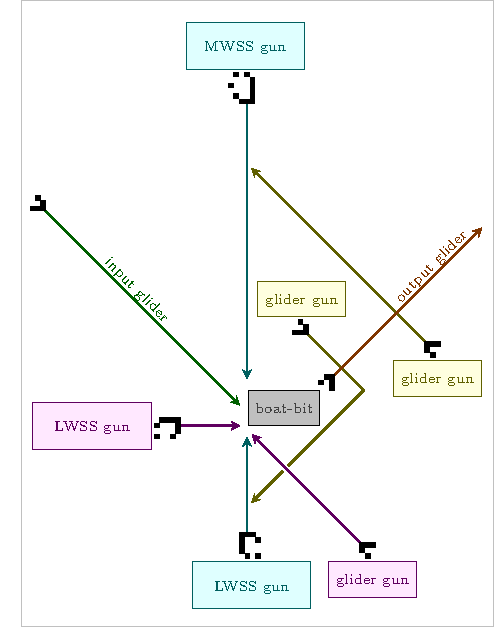
\includegraphics[width=1.062\textwidth]{periodic_circuitry/regulator_schematic.pdf}
		\caption{A schematic for a universal regulator.}
		\label{fig:universal_regulator_schematic}
	\end{subfigure} \ \ \ % 
	\begin{subfigure}{.485\textwidth}
		\centering\hspace*{-0.2cm}
		\patternimglink{0.081}{universal_regulator_periodic}
		\caption{A period~$60$ implementation of this regulator.}
		\label{fig:universal_regulator_periodic_real}
	\end{subfigure}
	\caption{A universal regulator's (a) schematic and (b) period~$60$ implementation. This device takes in a glider with \emph{any} timing from the northwest input lane (highlighted in \bgbox{greenpastel}{green}) and produces an output glider along the northeast lane with timing that is synchronized to some period (highlighted in \bgbox{orangeback2}{orange}). The left LWSS gun and bottom-right glider gun (highlighted in \bgbox{magentaback}{magenta}) are used to create the duoplet spark reaction from Figure~\ref{fig:make_sync_glider} that is at the heart of the regulator. The top MWSS gun and bottom LWSS gun (highlighted in \bgbox{aquaback}{aqua}) then rebuild the central eater~1 (thus allowing more input gliders), but only if the output glider has destroyed a glider from each of the suppressing glider streams (highlighted in \bgbox{yellowback2}{yellow}). These suppressing glider paths in the regulator (b) were adjusted for spacing reasons.}\label{fig:universal_regulator_periodic}
\end{figure}


%%%%%%%%%%%%%%%%%%%%%%%%%%%%%%%%
\section{Notes and Historical Remarks}\label{sec:periodic_circuits_notes}
%%%%%%%%%%%%%%%%%%%%%%%%%%%%%%%%

Because of their simplicity, many of the period~$30$ and period~$46$ mechanisms that we investigated in this chapter were discovered as early as the 1970s and '80s, so most of the earliest ``interesting'' patterns that were constructed in Conway's Game of Life make use of these components. Dean Hickerson built many of the most well-known of these constructions throughout the 1990s, including the first primer (which made use of essentially the same techniques, but slightly different components, as the one we constructed in Section~\ref{sec:primer}). Some other interesting constructions that he made mostly from these components include:\smallskip

\begin{itemize}
	\item A \emph{twin primer}\index{twin primer}---a gun that emits a stream of lightweight spaceships with the property that the $n$-th spaceship in the stream is present if and only if both $n-2$ and $n$ are prime (see Exercise~\ref{exer:twin_primer}). This pattern is particularly interesting since it is currently unknown whether or not there are infinitely many twin primes (in fact, this is one of the biggest open problems in all of mathematics), so it is unknown whether or not it emits infinitely many lightweight spaceships.\smallskip
	
	\item A pseudo-random glider generator based on using the toggle from Figure~\ref{fig:toggle} within a glider loop. If the output from a toggle is looped around and fed back into itself, the resulting stream of gliders ends up looking almost completely random as it turns itself off and on in increasingly erratic intervals. If we then place a glider duplicator somewhere on the loop, this random-looking stream of gliders can be emitted as an extremely high-period gun.
	
	Specifically, if there is space for $n$ gliders in the loop and we think of the $k$-th emitted glider as a bit $b(k)$ (where the $k$-th glider's presence means $b(k) = 1$ and its absence means $b(k) = 0$), then the effect of the toggle is that $b(k) = b(k-1) \oplus b(k-n)$ for all $k > n$.\footnote{Here, $\oplus$ refers to the XOR, or mod~$2$ addition, of two bits. That is, $0 \oplus 0 = 1 \oplus 1 = 0$ and $0 \oplus 1 = 1 \oplus 0 = 1$.} This sequence of bits is extremely erratic and can have very large period even when $n$ is relatively small \cite{A046932}. For example, the $n = 25$ case is illustrated in Figure~\ref{fig:prng_gun}, where the period of the sequence of bits is $10\,961\,685$ and thus the period of the gun itself is $30 \times 10\,961\,685 = 328\,850\,550$.\smallskip
%
%	Guns producing wildly different sequences of gliders and with wildly varying periods can be constructed by changing the length of the glider loop (see Exercise~\ref{exer:prng_gun}).\bigskip
	
	\begin{figure}[!htb]
		\centering
		\begin{subfigure}{.57\textwidth}
			\centering
			\patternimglink{0.095}{prng_gun}
			\caption{the pseudo-random gun}
		\end{subfigure} \ \ \ \ % 
		\begin{subfigure}{.39\textwidth}\vspace*{0.1cm}
			\texttt{1111111111111111111111111}\\
			\texttt{0101010101010101010101010}\\
			\texttt{0110011001100110011001100}\\
			\texttt{0100010001000100010001000}\\
			\texttt{0111100001111000011110000}\\
			\texttt{0101000001010000010100000}\\
			\texttt{0110000001100000011000000}\\
			\texttt{0100000001000000010000000}\\
			\texttt{0111111110000000011111111}\\
			\texttt{1010101011111111101010101}\\
			\texttt{0011001101010101001100110}\\
			\texttt{0010001001100110001000100}\\
			\texttt{0011110001000100001111000}\\
			\texttt{0010100001111000001010000\ensuremath{{}\, \cdots}}\vspace*{0.1cm}
			\caption{the first 400 bits of its output}
		\end{subfigure}
		\caption{A period $30 \times 10{\thousep}961{\thousep}685 = 328{\thousep}850{\thousep}550$ pseudo-random glider gun. It sends gliders around a $25 \times 30 = 750$-generation track (highlighted in \bgbox{aquaback}{aqua}) that contains a toggle (highlighted in \bgbox{greenpastel}{green}) and the glider duplication/inversion reaction introduced in Figure~\ref{fig:stream_inverter} (highlighted on the right in \bgbox{magentaback}{magenta}). By feeding the output of the toggle back into itself, the arrangement of $25$ gliders along the track becomes quite unpredictable and random-looking, and thus so does the output glider stream (highlighted in \bgbox{orangeback2}{orange}) that follows the $10{\thousep}961{\thousep}685$-bit string whose first $400$ bits are displayed in~(b).}\label{fig:prng_gun}
	\end{figure}
	
	\item A pattern that uses four breeders that aim Gosper glider guns so as to repeatedly invert each other and have asymptotic growth related to $\pi \approx 3.14159$. This pattern fills the plane with triangular regions that alternate back and forth between being filled and being empty.
	
	Specifically, if we use $T(n,t)$ to denote the triangle in the northeast quadrant with vertices at $(0,0)$ (i.e., the center of the pattern), $(0, t/(2n))$, and $(t/(2n+4), 0)$, then in generation~$t$ the triangle $T(1,t)$ is filled with gliders except that the smaller triangle $T(3,t)$ within it is empty, except that the smaller triangle $T(5,t)$ within it is filled with gliders, except that $T(7,t)$ is empty, and so on (see Figure~\ref{fig:life_computes_pi}).\bigskip
	
	\begin{figure}[!htb]
		\centering
		\embedlink{life_computes_pi}{\vcenteredhbox{\patternimg{0.113}{life_computes_pi_0}} \vcenteredhbox{\color{black}{$\xrightarrow{\text{\clock{12}{45} 4500}}$}} \vcenteredhbox{\patternimg{0.1394982181}{life_computes_pi_5000}}} % genarrow does not work with input as large as 5000
		\caption{An arrangement of four breeders (highlighted in \bgbox{yellowback2}{yellow}) that produce Gosper glider guns that fire at each other so as to invert each others' streams (shown on the left after the breeders have been moving away from each other for $500$~generations). In generation $t$ (shown here on the right with $t = 5000$), the \bgbox{greenpastel}{green} triangular region $T(1,t)$ is filled with gliders, except the \bgbox{aquaback}{aqua} triangular region $T(3,t)$ within it is empty, except the \bgbox{magentaback}{magenta} triangular region $T(5,t)$ within it is filled with gliders, and so on.}\label{fig:life_computes_pi}
	\end{figure}
	
	Since the triangle $T(n,t)$ has area
	\[
		A(n,t) = \frac{1}{2} \times \text{base} \times \text{height} = \frac{1}{2} \times \frac{t}{2n + 4} \times \frac{t}{2n} = \frac{t^2}{16} \left(\frac{1}{n} - \frac{1}{n+2}\right),
	\]
	the number of cells in the glider-filled portion of the Life plane in the northeast quadrant in generation~$t$ (when $t$ is large) is approximately
	\begin{align}\begin{split}\label{eq:triangle_alternate_area}
		A(1,t) - A(3,t) + A(5,t) - \cdots & = \frac{t^2}{16} \left( \left(1 - \frac{1}{3}\right) - \left(\frac{1}{3} - \frac{1}{5}\right) + \left(\frac{1}{5} - \frac{1}{7}\right) - \cdots\right) \\
		& = \frac{t^2}{16} \left( 1 - \frac{2}{3} + \frac{2}{5} - \frac{2}{7} + \cdots\right).
	\end{split}\end{align}
	If we use the fact that $\arctan(x)$ has Taylor series $\arctan(x) = x - x^3/3 + x^5/5 - \cdots$, we learn that $\arctan(1) = 1 - 1/3 + 1/5 - \cdots$. If we also use the fact that $\arctan(1) = \pi/4$, and combine these equalities with the sum~\eqref{eq:triangle_alternate_area}, we learn that the occupied area in the northeast quadrant contains roughly
	\begin{align*}
		\frac{t^2}{16} \left( 1 - \frac{2}{3} + \frac{2}{5} - \frac{2}{7} + \cdots\right) = \frac{t^2}{16}\big( 2\arctan(1) - 1\big) = \frac{(\pi-2)t^2}{32}
	\end{align*}
	cells (when $t$ is large). Since the gliders fill this occupied area with density $1/90$, and this same calculation applies to all four quadrants of the plane, we see that this pattern's population in generation~$t$ (again, when $t$ is large) is approximately
	\[
		\frac{4}{90} \times \frac{(\pi-2)t^2}{32} = \frac{(\pi-2)t^2}{720}.
	\]
\end{itemize}

In fact, John Conway and Bill Gosper used little more than some basic period~$30$ circuitry way back in the 1970s and 1980s \cite[Chapter~25]{BCG82} to demonstrate that the Game of Life is \emph{universal}---anything that can be computed (by a regular computer, for example), can be computed in the Game of Life by cleverly arranging some period~$30$ circuitry and manipulating gliders. Thus, for example, we knew that prime numbers could be computed in the Game of Life for several years before the first primer was explicitly constructed.

The advantage of the new circuitry and constructions that we have available to us now is that they are significantly smaller than the ones that would result from implementing the construction outlined by Conway and Gosper's universality proof \index{computational universality} (which require sending gliders across absolutely vast distances for even the simplest of computations). There is also something quite appealing about having \emph{explicit} constructions of these patterns. Actually arranging components as required by Conway and Gosper's proofs would typically be infeasible in practice, and the resulting patterns would not be terribly interesting to look at. We'll return to the topic of computational universality in Chapter~\ref{chp:universal_computation}.


%%%%%%%%%%%%%%%%%%%%%%%%%%%%%%%%%
\section*{Exercises \hfill \normalfont\textsf{\small solutions to starred exercises on \hyperlink{solutions_periodic_circuitry}{page \pageref{solutions_periodic_circuitry}}}}
\label{sec:periodic_exercises}
\addcontentsline{toc}{section}{Exercises}
\vspace*{-0.4cm}\hrulefill\vspace*{-0.3cm}\footnotesize\begin{multicols}{2}\vspace*{-0.4cm}\raggedcolumns\interlinepenalty=10000
\setlength{\parskip}{0pt}
%%%%%%%%%%%%%%%%%%%%%%%%%%%%%%%%%
	
	
	\begin{problemstar}\label{exer:inline_inverter_gun_why_buckaroo} \probdiff{1}
		In the glider gun in Figure~\ref{fig:inline_inverter_p120_gun}, we used eater~1s instead of blocks to stabilize some of the Gosper glider guns (as in the buckaroo of Figure~\ref{fig:buckaroo}). Explain why.
	\end{problemstar}
	
	
	\mfilbreak
	
	
	\begin{problem}\label{exer:inline_inverter_gun_high_period} \probdiff{1}
		Construct a glider gun based on the inline inverter with...\smallskip
		
		\begin{enumerate}[label=\bf\color{ocre}(\alph*)]
			\item period~$240$.
			
			\item period~$360$.
		\end{enumerate}
	\end{problem}
% SOLUTION: Some of these are given in our primer.
	
	
	\mfilbreak
	
	
	\begin{problem}\label{exer:inline_inverter_advancer} \probdiff{2}
		Use two inline inverters to create a pattern that advances a stream of gliders by $20$ generations, similar to how the fast forward force field\index{fast forward force field} of Figure~\ref{fig:fast_forward_force_field} advances a stream of lightweight spaceships.
	\end{problem}
	% SOLUTION: Signal-circuitry/advancer.rle uses 6 inline inverters to advance gliders quicker than c/4
	
	
	\mfilbreak
	
	
	\begin{problem}\label{exer:inline_inverter_lwss_gun} \probdiff{2}
		Construct a period~$240$ lightweight spaceship gun...\smallskip
		
		\begin{enumerate}[label=\bf\color{ocre}(\alph*)]
			\item using three inline inverter guns.
			
			\item using one inline inverter gun and the reaction from Figure~\ref{fig:glider_to_lwss}.
		\end{enumerate}
	\end{problem}
	
	
	\mfilbreak
	
	
	\begin{problem}\label{exer:glider_to_hwss_to_glider}
		The periodic circuits displayed below can be used to convert two gliders into an HWSS and an HWSS back into a glider.\footnote{These reactions were found and simplified by David Buckingham, Bill Gosper, Dieter Leithner, and Peter Rott.}
		\begin{center}
			\patternimglink{0.12}{glider_to_hwss_to_glider}
		\end{center}
		\begin{enumerate}[label=\bf\color{ocre}(\alph*)]
			\item \probdiff{2} Use the left reaction to create a period~$120$ HWSS gun.
			
			\item \probdiff{3} Create a glider loop that uses both of these reactions to convert a glider into an HWSS and back.
		\end{enumerate}
	\end{problem}
	% (b) solution:
	%x = 80, y = 42
	%47b2o$47bo$35bo9bobo$33bobo9b2o$32bobo$26b2o3bo2bo$26b2o4bobo$33bobo$
	%35bo3$32b2o$32bo$23bo6bobo$23bobo4b2o3bo$6b2o18b2o6bo$4bo3bo17b2o6b3o$
	%3bo5bo16b2o$2b2obo3bo8bo4bobo$3bo5bo9bo3bo$4bo3bo5bo2b3o$6b2o2$3bo$2bo
	%bo$bo3bo$2b3o21bo$2o3b2o17bobo45bo4bo$25b2o43b2ob4ob2o$72bo4bo2$15b2ob
	%2obo$14b2o2b2ob2o$22bo41bo2bo$14b2o51bo$14b2o5b2o4b2o34bo4bo$21b2o3bob
	%o5b2o27b2o2bobo$14bo12bo6bo33bob2o$3b2o9b2ob2o2b2o12b3o$3b2o10bob2ob2o
	%15bo$68bo2bo$68b2o!
	
	
	\mfilbreak
	
	
	\begin{problem}\label{exer:any_wss_to_glider}
		The arrangement of queen bees below can be used to convert any xWSS into a glider.
		\begin{center}
			\patternimglink{0.1}{any_wss_to_glider}
		\end{center}
		\begin{enumerate}[label=\bf\color{ocre}(\alph*)]
			\item \probdiff{3} Use this reaction as well as one of the reactions from Exercise~\ref{exer:glider_to_hwss_to_glider} to create a glider loop that converts a glider into an HWSS and back.
			
			\item \probdiff{1} Use this reaction to create a gun that emits a glider stream (rather than an LWSS stream as in Figure~\ref{fig:primer}) that is spaced according to the prime numbers.
		\end{enumerate}
	\end{problem}
	
	
	\mfilbreak
	
	
	\begin{problem}\label{exer:glider_to_lwss_loop} \probdiff{2}
		Construct an oscillator that makes use of the reactions in each of Figures~\ref{fig:glider_to_lwss} and~\ref{fig:lwss_to_glider} to send a glider around a track in such a way that it is converted into an LWSS and back during each loop.
	\end{problem}
	% SOLUTION:
	%x = 73, y = 52, rule = B3/S23
	%29b2o19b2o$30bo19bo$30bobo8bo6bobo$31b2o5b4o6b2o$37b4o$37bo2bo$37b4o$
	%38b4o$41bo2$38bo$36bobo$37b2o5$21bo$21b2o$20bobo3$4b2o$2bo4bo$bo6bo$o
	%8bo43bo$o8bo41bobo$o8bo15b4o23b2o6b2o$bo6bo16bo3bo30bobo$2bo4bo17bo29b
	%2o6bo$4b2o20bo2bo24bo2bo2bo2bo7b2o$16bo38b2o6bo7b2o$16bo43bobo$15b3o
	%42b2o2$55b3o$15b3o37b3o$16bo37bo3bo$16bo36bo5bo$16bo37bo3bo$16bo38b3o$
	%15b3o3$15b3o$16bo$16bo4$56b2o$56b2o!
	
	
	\mfilbreak
	
	
	\begin{problem}\label{exer:period_not_235_gun} \probdiff{3}
		Construct a pattern that emits a stream of lightweight spaceships with the property that the $n$-th spaceship in the stream is present if and only if $n$ is not a multiple of $2$, $3$, or $5$.
	\end{problem}
	
	
	\mfilbreak
	
	
	\begin{problem}\label{exer:twin_primer} \probdiff{3}
		The collision of a glider with an LWSS shown below is called a \emph{filter}\index{filter}. It results in a single block that destroys the next incoming glider, letting the next incoming LWSS pass by unharmed, thus doubling the period of an LWSS stream.
		
		\begin{center}
			\embedlink{exercise_lwss_filter}{\vcenteredhbox{\patternimg{0.1}{exercise_lwss_filter_0}} \vcenteredhbox{\genarrow{6}} \vcenteredhbox{\patternimg{0.1}{exercise_lwss_filter_6}}}
		\end{center}
		
		\noindent Add this reaction (and potentially some guns and eaters, as necessary) to the primer to create a \emph{twin primer}\index{twin primer}---a pattern that creates a stream of lightweight spaceships for which the $n$-th LWSS in the stream is present if and only if $n-2$ and $n$ are both prime.
	\end{problem}


	\mfilbreak
	
	
	\begin{problem}\label{exer:rewind_primer} \probdiff{4}
		One method of making a pattern smaller is to change it into the form that it would have looked several generations earlier (this is called \emph{rewinding}\index{rewind} the pattern). Use this technique, along with moving its various components closer together, to reduce the area of the bounding box of the primer from Figure~\ref{fig:primer} from $951 \times 696 = 661{\thousep}896$ to $500{\thousep}000$ or less.
	\end{problem}
	
	
	\mfilbreak
	
	
	\begin{problem}\label{exer:twin_bees_loop} \probdiff{2}
		Use the patterns from Figure~\ref{fig:twin_bees_reflect} to create a loop oscillator in which a glider is converted into a lightweight spaceship and back at some point in the loop.
	\end{problem}
	
	
	\mfilbreak
	
	
	\begin{problem}\label{exer:twin_bees_mwss_gun} \probdiff{2}
		Use the patterns from Figure~\ref{fig:twin_bees_weird_guns} to construct a period~$46$ middleweight spaceship gun.
	\end{problem}
	
	
	\mfilbreak
	
	
	\begin{problem}\label{exer:ticker_tape_gun_store_different} \probdiff{1}
		Modify the sequence of gliders in the loop of the gun from Figure~\ref{fig:ticker_tape_gun} so that it produces lightweight spaceships corresponding to the bitstring ``110111010011011101001''.
	\end{problem}


	\mfilbreak
	
	
	\begin{problem}\label{exer:p30_ticker_tape_gun} \probdiff{3}
		Rebuild the ticker tape gun from Figure~\ref{fig:ticker_tape_gun} so that it uses p$30$ circuitry instead of p$46$. Relevant mechanisms can be found in Figures~\ref{fig:periodic_glider_duplicator} and~\ref{fig:glider_to_lwss}.
	\end{problem}
	
	
	\mfilbreak
	
	
	\begin{problem}\label{exer:ticker_tape_smiley_gun} \probdiff{3}
		Using the techniques used in Figure~\ref{fig:ticker_tape_hi_gun}, create a ticker tape gun that produces smiley faces.
	\end{problem}
	
	
	\mfilbreak
	
	
	\begin{problem}\label{exer:ticker_tape_gun_memory_alter} \probdiff{2}
		Fire some gliders at the memory cell\index{memory cell} from Figure~\ref{fig:p46_memory_cell} so as to change the bitstring that it stores to ``101010101010''.
	\end{problem}
	
	
	\mfilbreak
	
	
	\begin{problem}\label{exer:tanners_p46_twin_bee_gun} \probdiff{3}
		Create a glider gun that works by colliding the spark from Tanner's p$46$ with a twin bees shuttle that is stabilized only on one side.
		
		\noindent [Hint: This gun can be found by hand via trial and error, or you could write a computer program to try lots of positionings.]
	\end{problem}
	% NOTE: Found by David Bell
	% SOLUTION:
	%x = 31, y = 44
	%17boo5boo$17boo5boo11$17bo7bo$15boboo5boobo$15bo3booboo3bo$16bo3bobo3b
	%o$17b3o3b3o10$14bo14bo$13b3o14bo$12bobobo11b3o$12bobobo$10boob3oboo$9b
	%obooboboobo$3boo3boobo5boboo$3boo4boobo3boboobboboo$10b3o3b3o3boobo$$
	%bboo$3bo$3o$o13bo$13boboboboo$12bobooboobo$12bo$11boo!
	
	
	\mfilbreak
	
	
	\begin{problem}\label{exer:tanners_p46_reflect} \probdiff{3}
		Show how Tanner's p$46$ can be used to reflect a glider by 180~degrees.
		
		\noindent [Hint: The spark emitted by Tanner's p$46$ is quite similar to some of the sparks emitted by the pentadecathlon. Mimic the reflection from Figure~\ref{fig:p30_relay}.]
	\end{problem}
	% NOTE: Found by David Bell
	% SOLUTION:
	%x = 209, y = 182
	%201b8o$201bob4obo$201b8o155$4boo$5bo28boo$5bobo25bobo$6boobboo23bo$10b
	%oo7$o$3o7boo$3bo6boo$bbobo7bo$bboo6boo$10boo$bboo$bbo$3b3o$5bo$8boo$9b
	%o$6b3o$6bo!
	
	
	\mfilbreak
	
	
	\begin{problem}\label{exer:twin_bees_large_spark}
		An arrangement of two twin bees shuttles that is particularly useful due to the extremely large spark that it produces is displayed below.
		
		\begin{center}
			\patternimglink{0.1}{twin_bees_large_spark}
		\end{center}
		
		\begin{enumerate}[label=\bf\color{ocre}(\alph*)]
			\item \probdiff{3} Collide the spark from this object with that of Tanner's p$46$ to create a glider gun.
			
			\noindent [Hint: Writing a computer program might be helpful here.]
			
			\item \probdiff{4} Collide the spark from this object with the large-spark version of the twin bees shuttle from Figure~\ref{fig:twin_bees_reflect} so as to create a double-barreled glider gun\index{double-barreled gun} (i.e., a gun that emits two side-by-side gliders per period).\footnote{This double-barreled gun was originally found by Dieter Leithner.}
		\end{enumerate}
	\end{problem}
	% Shows up in vaccuum gun and also p46 gliderless HWSS gun (twice)
	% Solution for (a), but there are at least 6 others too:
	%28b2o$28bo$26bobo$17b2o7b2o$2o14b2ob2o$2o15bo2bo$17bo2bo$18b2o2$18b2o$
	%17bo2bo$2o15bo2bo$2o14b2ob2o12b2o14b2o$17b2o13b2o15b2o$33b5o$34b4o2$
	%34b4o$33b5o$32b2o15b2o$33b2o14b2o14$21bo$20b3o$19b5o$18b2o3b2o$17b2o5b
	%2o5b2o$18b2o3b2o6b2o$13b2o4bo3bo$12bobo$12bo19b2o$11b2o19bo$33b3o$21bo
	%13bo$15b2obobobo$15bob2ob2obo$23bo$23b2o!
	% Solution for (b):
	%b2o23b2o$b2o23bo$24bobo$8b2o14b2o$2o5bobo$2o5bo$7b3o$23b2o$25bo18b2o$
	%21bo2b2o18b2o$7b3o10b3obo9bo$2o5bo12bo3bo7bo2bo$2o5bobo9b5o8b5o8b2o$8b
	%2o10bob3obo5b3ob2o7b2o$20b2obo3bo5b2obo$b2o21bobo7b2o$b2o21b2o$22b2o
	%10b2o$21bo2bo8b2obo$24bo7b3ob2o7b2o$21bo2bo7b5o8b2o$22b3o7bo2bo$34bo$
	%44b2o$44b2o5$31bo$30b2o15b2o$29b2o16b2o$30b2o2b2o4$30b2o2b2o$29b2o16b
	%2o$30b2o15b2o$16b2o13bo$15bobo$15bo$14b2o!
	
	
	\mfilbreak
	
	
	\begin{problem}\label{exer:2eng_corder_gun} \probdiff{3}
		Use the $9$-glider synthesis from Exercise~\ref{exer:2_engine_cordership_synthesis} to construct a gun that fires $2$-engine Corderships.
		
		\noindent [Hint: Start off by choosing an appropriately large period. Corderships cannot follow behind each other at period~30 or~46, for example, so you need to use larger-period guns.]
	\end{problem}
	% Numerous possible solutions here: https://www.conwaylife.com/forums/viewtopic.php?t=&p=54750#p54750
	
	
	\mfilbreak
	
	
	\begin{problem}\label{exer:mwss_out_of_blue_double_period} \probdiff{3}
		Construct a p46 LWSS gun, and then apply an MWSS out of the blue to its output to turn it into a p92 LWSS gun.
		
		\noindent [Hint: The MWSS that the MWSS out of the blue reaction produces can collide with an LWSS so that they cleanly destroy each other.]
	\end{problem}
% SOLUTION (by Dean Hickerson April 1998):
%x = 170, y = 57, rule = B3/S23
%153bo3bo$152bo5bo9b2o$135bo16bo15b2o$133bo2bo15b2o3bo$121b2o10b5o16b3o
%$121b2o10b3ob2o$134b2obo16b3o$135b2o15b2o3bo$152bo15b2o$125b2o8b2o15bo
%5bo9b2o$123bob3o6b2obo15bo3bo$121b3o4bo4b3ob2o$123bob3o5b5o$125b2o6bo
%2bo$135bo17bo$154b2o$bo2bo88bo2bo42bo2bo10b2o13b2o$o91bo45bo23bo5b2o$o
%3bo37bo49bo3bo41bo3bo18b3o$4o36bo3bo47b4o42b4o18bo3bo$45bo100b2o12b2ob
%2o$40bo4bo98bo2bo$41b5o97b2o2bo13b3o$25b2o116bo2bo14b3o$14b3o8bob2o54b
%2o8b3o34b2o11bobo$2o11bo4bo6bob2o53bo2bo6b2obo32b2ob2o$2o10bo5bo6bobo
%53b2o2bo5bobobo32bo2bo11bo2bo$13bo9bob2o55bo2bo6bo35bo2bo11bo2bo$14b2o
%7b2o8b2o48bo7bobo7b2o26b2o22b2o$33b2o66b2o41b2o7b2o8b2ob2o$14b2o67bo8b
%o36b2o32b2ob2o$13bo8b2o58bo2bo4bo37bo2bo11bobo17b2ob2o$2o10bo5bo3b2o
%44b2o11b2o2bo4b2o28b2o6bo2bo11bobo15bob2ob2obo$2o11bo4bo49b2o12bo2bo
%34b2o6b2ob2o28b3o3b3o$14b3o66b2o45b2o30bo5bo4$146b3o3b3o$146bo2bobo2bo
%$146bo7bo2$26b2o5b2o59b2o5b2o44bo5bo$26bob2ob2obo58bo2bo3bo2bo44b2ob2o
%8b2o5b2o$27bobobobo60bo2bobo2bo58b2o5b2o$27bobobobo63bobo$26bo7bo60b3o
%b3o$93b3o5b3o$93b2o7b2o$93b2o7b2o$28b2ob2o61bob2ob2obo$26bo2bobo2bo59b
%3o3b3o$26b3o3b3o60bo5bo$27bo5bo2$26b2o5b2o59b2o5b2o43b2o5b2o$26b2o5b2o
%59b2o5b2o43b2o5b2o!
	
	
	\mfilbreak
	

	\begin{problem}\label{exer:construct_p30_heisenburp} \probdiff{4}
		Construct a version of the Heisenburp from Figure~\ref{fig:p46_heisenburp_constructed} that uses period~$30$ circuitry instead of period~$46$.
	\end{problem}
	
	
	\mfilbreak
	
	
	\begin{problemstar}\label{exer:bumper_bouncer_wrong_color} \probdiff{1}
		Explain why it is not possible to construct glider loop oscillators consisting only of the following sets of reflectors, and experiment with them to convince yourself that they really are impossible.\smallskip
		
		\begin{enumerate}[label=\bf\color{ocre}(\alph*)]
			\item Three bumpers and one bouncer.
			
			\item Three bouncers and one Snark.
		\end{enumerate}
	\end{problemstar}
	
	
	\mfilbreak
	
	
	\begin{problemstar}\label{exer:bumper_high_period}
		Construct a bumper reflector with...\smallskip
		
		\begin{enumerate}[label=\bf\color{ocre}(\alph*)]
			\item \probdiff{1} period~$16$.
			
			\item \probdiff{1} period~$22$.
			
			\item \probdiff{1} period~$4$, making use of the fountain\index{fountain} sparker.
			
			\item \probdiff{2} period~$15$.
			
			\item \probdiff{3} period~$5$.
			
			\noindent [Hint: Modify the sparker from Figure~\ref{fig:p5_bouncer}.]
		\end{enumerate}
	\end{problemstar}


	\mfilbreak
	
	
	\begin{problemstar}\label{exer:p29_pipsquirter} \probdiff{2}
		Use the \emph{skewed p$29$ pre-pulsar shuttle}\index{pre-pulsar shuttle} displayed below to create a p$29$ bouncer reflector.\footnote{This reflector was originally found by Matthias Merzenich in August 2013.}
		
		\begin{center}
			\patternimglink{0.1}{skewed_p29}
		\end{center}
	\end{problemstar}


	\mfilbreak
	
	
	\begin{problem}\label{exer:make_inline_inverter_with_weird_period} \probdiff{3}
		Use the reaction from Figure~\ref{fig:stream_inverter}, together with reflectors and eaters as necessary, to create a device that duplicates and inverts a glider stream with...\smallskip
		
		\begin{enumerate}[label=\bf\color{ocre}(\alph*)]
			\item period~$43$.
			
			\item period~$36$.
			
			\item period~$25$.
		\end{enumerate}
	\end{problem}
	
	
	\mfilbreak
	
	
	\begin{problemstar}\label{exer:p11_bumper_not_useful} \probdiff{2}
		Explain why the period~$11$ bumper from Figure~\ref{fig:p11_bumper} is not particularly useful for glider streams of period below $121$.
		
		\noindent [Hint: There are smaller reflectors that can be used in its place.]
	\end{problemstar}
	
	
	\mfilbreak
	
	
	\begin{problemstar}\label{exer:minimum_period_snark_loop}
		The smallest-period single-glider Snark loop has period~$216$ and is displayed in Figure~\ref{fig:minimum_snark_loop}. Note that the still life in the center of this loop is the weld of four eater~1s from Exercise~\ref{exer:eater_weld}(c).\smallskip
		
		\begin{enumerate}[label=\bf\color{ocre}(\alph*)]
			\item \probdiff{1} Move each of the Snarks outward by $1$~cell (e.g., move the northern Snark north by $1$ cell) and un-weld the central eater~$1$s. What is the period of the resulting glider loop? Explain how you could have determined this period without explicitly constructing this modified glider loop.
			
			\item \probdiff{2} Replace the Snarks in the glider loop from part~(a) by p$4$~bumpers in a way that keeps the glider on the same lanes. What is the period of the resulting glider loop? Explain how you could have determined this period without explicitly constructing this modified glider loop.
			
			\item \probdiff{1} Replace one of the p$4$ bumpers in the glider loop from part~(b) with a p$6$ bumper.
			
			\item \probdiff{1} If you replace one of the p$4$ bumpers in the glider loop from part~(b) with a p$5$ bumper, the loop stops working. Why?
			
			\item \probdiff{2} Move some of the bumpers in the glider loop from part~(b) closer together so as to alter the period of the loop. Once you have made a loop with a suitable period, replace one of the p$4$ bumpers by a p$5$ bumper.
			
			\noindent\begin{center}
				\patternimglink{0.08}{minimum_snark_loop}
			\end{center}
		\end{enumerate}
	\end{problemstar}
	
	
	\mfilbreak
	
	
	\begin{problemstar}\label{exer:p60_regulator_mwss_emulator} \probdiff{2}
		The lightweight spaceship guns in Figure~\ref{fig:universal_regulator_periodic_real} each contain a middleweight emulator. Describe what role this oscillator plays in the gun.
	\end{problemstar}
	
	
	\mfilbreak
	
	
	\begin{problem}\label{exer:p60_regulator_reflectors} \probdiff{2}
		There are two reflectors in Figure~\ref{fig:universal_regulator_periodic_real} that reflect yellow glider streams. What are the names of these reflectors (we have discussed them each earlier)?
	\end{problem}


	\mfilbreak
	
	
	\begin{problem}\label{exer:universal_regulator_repeat_time} \probdiff{2}
		What is the repeat time of the universal regulator from Figure~\ref{fig:universal_regulator_periodic_real}? Explain why it is not~$60$.
	\end{problem}
% SOLUTION: 355. Not 60 because we have to wait for the output signal to trigger the reconstruction of the central eater 1.
	
	
	\mfilbreak
	
	
	\begin{problemstar}\label{exer:prng_gun}
		Changing the number of gliders in the loop portion of the pseuro-random glider-generating gun from Figure~\ref{fig:prng_gun} can drastically change its period.\smallskip
		
		\begin{enumerate}[label=\bf\color{ocre}(\alph*)]
			\item \probdiff{1} If you move the northwest portion of the loop northwest by an additional $15$~cells (and rephase reflectors as necessary), how many additional gliders fit in the loop?
			
			\item \probdiff{3} Determine the period of the gun constructed in part~(a). [Hint: The period is massive. Use computer software to help you and/or compute the period from the recurrence relation given in the text.]
			
			\item \probdiff{2} Move the northwest portion of the loop northwest by an \emph{additional} $15$~cells (again, rephase reflectors as necessary). Determine the period of this gun. [Hint: Its period is now small enough that you \emph{may} be able to compute it by hand if you are clever.]
		\end{enumerate}
	\end{problemstar}
	
	% EXERCISE: Use this glider-producing collision to make a p23 glider gun via stream merging:
	%x = 68, y = 34, rule = B3/S23
	%39bo$b2o27b3o$b2o18b2o5bo4bo11b2o$28bo5bo10b2o$13b2o18bo$2o9b2o2bo15b
	%2o$2o9b6o$11b4o16b2o$24bo8bo$25bo2bo5bo$23b3o2bo4bo31b2o$11b4o15b3o32b
	%2o$2o9b6o$2o9b2o2bo$13b2o26b2o8b3o12b2o$41b2o8bo3bo10b2o$b2o48bo4bo$b
	%2o49bo3bo2$52bo3bo$36bo14bo4bo$34bobo14bo3bo10b2o$24bo10b2o14b3o12b2o$
	%7b2o15b2o$7b2o16b2o$20b2o2b2o39b2o$40bobo22b2o$41b2o$41bo$20b2o2b2o$7b
	%2o16b2o7b2o$7b2o15b2o8b2o11bo$24bo23bo$46b3o!
	
	
	% EXERCISE: create a p23 glider gun using this reflection
	%x = 38, y = 49, rule = B3/S23
	%22bo$23bo$21b3o3$29bo$29bobo$29b2o$25b2o$10b2o13b2o$2o6b2ob2o11b3o$2o
	%6bo2bo9bob4o$8bo2bo8bo4bo$9b2o14bo$24bo$9b2o$8bo2bo10b2o$8bo2bo$8b2ob
	%2o$10b2o$34b2o$34b2o8$28bo5bo$27b3o3b3o$26b2obo3bob2o3$29bo3bo$29bo3bo
	%5$34bo$33bobo$32b2ob2o$32bo3bo$31b3ob3o$32bo3bo$32bo3bo$27b2o4bobo$27b
	%2o5bo!
	
	% EXERCISE: Construct a p46 glider duplicator
	
	% p46 ege shooter based on twin bees?
	%x = 67, y = 82, rule = B3/S23
	%3$47b2o5b2o$47b2o5b2o7$48bo5bo$47b3o3b3o$46bo2b2ob2o2bo$46b3o5b3o9$47b
	%3o$46bo3bo$46b2ob2o$47bobo2$47bobo$46b2ob2o$46bo3bo3b2o$47b3o4b2o2$39b
	%obo2b2o$24b2o12bo3bob3o$24b2o13bo6b2o$40b5obo$43b3o2$43b3o$40b5obo$24b
	%2o13bo6b2o$24b2o12bo3bob3o$39bobo2b2o7$38bobo$38b2o$39bo9$28bo$26b2o$
	%27b2o10$15bobo$15b2o$16bo!
	
	%% EXERCISE END COMMANDS
\end{multicols}
\normalsize\vspace*{0.01cm}
%% DONE EXERCISE END COMMANDS